\documentclass[11pt]{article}

    \usepackage[breakable]{tcolorbox}
    \usepackage{parskip} % Stop auto-indenting (to mimic markdown behaviour)
    

    % Basic figure setup, for now with no caption control since it's done
    % automatically by Pandoc (which extracts ![](path) syntax from Markdown).
    \usepackage{graphicx}
    % Maintain compatibility with old templates. Remove in nbconvert 6.0
    \let\Oldincludegraphics\includegraphics
    % Ensure that by default, figures have no caption (until we provide a
    % proper Figure object with a Caption API and a way to capture that
    % in the conversion process - todo).
    \usepackage{caption}
    \DeclareCaptionFormat{nocaption}{}
    \captionsetup{format=nocaption,aboveskip=0pt,belowskip=0pt}

    \usepackage{float}
    \floatplacement{figure}{H} % forces figures to be placed at the correct location
    \usepackage{xcolor} % Allow colors to be defined
    \usepackage{enumerate} % Needed for markdown enumerations to work
    \usepackage{geometry} % Used to adjust the document margins
    \usepackage{amsmath} % Equations
    \usepackage{amssymb} % Equations
    \usepackage{textcomp} % defines textquotesingle
    % Hack from http://tex.stackexchange.com/a/47451/13684:
    \AtBeginDocument{%
        \def\PYZsq{\textquotesingle}% Upright quotes in Pygmentized code
    }
    \usepackage{upquote} % Upright quotes for verbatim code
    \usepackage{eurosym} % defines \euro

    \usepackage{iftex}
    \ifPDFTeX
        \usepackage[T1]{fontenc}
        \IfFileExists{alphabeta.sty}{
              \usepackage{alphabeta}
          }{
              \usepackage[mathletters]{ucs}
              \usepackage[utf8x]{inputenc}
          }
    \else
        \usepackage{fontspec}
        \usepackage{unicode-math}
    \fi

    \usepackage{fancyvrb} % verbatim replacement that allows latex
    \usepackage{grffile} % extends the file name processing of package graphics
                         % to support a larger range
    \makeatletter % fix for old versions of grffile with XeLaTeX
    \@ifpackagelater{grffile}{2019/11/01}
    {
      % Do nothing on new versions
    }
    {
      \def\Gread@@xetex#1{%
        \IfFileExists{"\Gin@base".bb}%
        {\Gread@eps{\Gin@base.bb}}%
        {\Gread@@xetex@aux#1}%
      }
    }
    \makeatother
    \usepackage[Export]{adjustbox} % Used to constrain images to a maximum size
    \adjustboxset{max size={0.9\linewidth}{0.9\paperheight}}

    % The hyperref package gives us a pdf with properly built
    % internal navigation ('pdf bookmarks' for the table of contents,
    % internal cross-reference links, web links for URLs, etc.)
    \usepackage{hyperref}
    % The default LaTeX title has an obnoxious amount of whitespace. By default,
    % titling removes some of it. It also provides customization options.
    \usepackage{titling}
    \usepackage{longtable} % longtable support required by pandoc >1.10
    \usepackage{booktabs}  % table support for pandoc > 1.12.2
    \usepackage{array}     % table support for pandoc >= 2.11.3
    \usepackage{calc}      % table minipage width calculation for pandoc >= 2.11.1
    \usepackage[inline]{enumitem} % IRkernel/repr support (it uses the enumerate* environment)
    \usepackage[normalem]{ulem} % ulem is needed to support strikethroughs (\sout)
                                % normalem makes italics be italics, not underlines
    \usepackage{soul}      % strikethrough (\st) support for pandoc >= 3.0.0
    \usepackage{mathrsfs}
    

    
    % Colors for the hyperref package
    \definecolor{urlcolor}{rgb}{0,.145,.698}
    \definecolor{linkcolor}{rgb}{.71,0.21,0.01}
    \definecolor{citecolor}{rgb}{.12,.54,.11}

    % ANSI colors
    \definecolor{ansi-black}{HTML}{3E424D}
    \definecolor{ansi-black-intense}{HTML}{282C36}
    \definecolor{ansi-red}{HTML}{E75C58}
    \definecolor{ansi-red-intense}{HTML}{B22B31}
    \definecolor{ansi-green}{HTML}{00A250}
    \definecolor{ansi-green-intense}{HTML}{007427}
    \definecolor{ansi-yellow}{HTML}{DDB62B}
    \definecolor{ansi-yellow-intense}{HTML}{B27D12}
    \definecolor{ansi-blue}{HTML}{208FFB}
    \definecolor{ansi-blue-intense}{HTML}{0065CA}
    \definecolor{ansi-magenta}{HTML}{D160C4}
    \definecolor{ansi-magenta-intense}{HTML}{A03196}
    \definecolor{ansi-cyan}{HTML}{60C6C8}
    \definecolor{ansi-cyan-intense}{HTML}{258F8F}
    \definecolor{ansi-white}{HTML}{C5C1B4}
    \definecolor{ansi-white-intense}{HTML}{A1A6B2}
    \definecolor{ansi-default-inverse-fg}{HTML}{FFFFFF}
    \definecolor{ansi-default-inverse-bg}{HTML}{000000}

    % common color for the border for error outputs.
    \definecolor{outerrorbackground}{HTML}{FFDFDF}

    % commands and environments needed by pandoc snippets
    % extracted from the output of `pandoc -s`
    \providecommand{\tightlist}{%
      \setlength{\itemsep}{0pt}\setlength{\parskip}{0pt}}
    \DefineVerbatimEnvironment{Highlighting}{Verbatim}{commandchars=\\\{\}}
    % Add ',fontsize=\small' for more characters per line
    \newenvironment{Shaded}{}{}
    \newcommand{\KeywordTok}[1]{\textcolor[rgb]{0.00,0.44,0.13}{\textbf{{#1}}}}
    \newcommand{\DataTypeTok}[1]{\textcolor[rgb]{0.56,0.13,0.00}{{#1}}}
    \newcommand{\DecValTok}[1]{\textcolor[rgb]{0.25,0.63,0.44}{{#1}}}
    \newcommand{\BaseNTok}[1]{\textcolor[rgb]{0.25,0.63,0.44}{{#1}}}
    \newcommand{\FloatTok}[1]{\textcolor[rgb]{0.25,0.63,0.44}{{#1}}}
    \newcommand{\CharTok}[1]{\textcolor[rgb]{0.25,0.44,0.63}{{#1}}}
    \newcommand{\StringTok}[1]{\textcolor[rgb]{0.25,0.44,0.63}{{#1}}}
    \newcommand{\CommentTok}[1]{\textcolor[rgb]{0.38,0.63,0.69}{\textit{{#1}}}}
    \newcommand{\OtherTok}[1]{\textcolor[rgb]{0.00,0.44,0.13}{{#1}}}
    \newcommand{\AlertTok}[1]{\textcolor[rgb]{1.00,0.00,0.00}{\textbf{{#1}}}}
    \newcommand{\FunctionTok}[1]{\textcolor[rgb]{0.02,0.16,0.49}{{#1}}}
    \newcommand{\RegionMarkerTok}[1]{{#1}}
    \newcommand{\ErrorTok}[1]{\textcolor[rgb]{1.00,0.00,0.00}{\textbf{{#1}}}}
    \newcommand{\NormalTok}[1]{{#1}}

    % Additional commands for more recent versions of Pandoc
    \newcommand{\ConstantTok}[1]{\textcolor[rgb]{0.53,0.00,0.00}{{#1}}}
    \newcommand{\SpecialCharTok}[1]{\textcolor[rgb]{0.25,0.44,0.63}{{#1}}}
    \newcommand{\VerbatimStringTok}[1]{\textcolor[rgb]{0.25,0.44,0.63}{{#1}}}
    \newcommand{\SpecialStringTok}[1]{\textcolor[rgb]{0.73,0.40,0.53}{{#1}}}
    \newcommand{\ImportTok}[1]{{#1}}
    \newcommand{\DocumentationTok}[1]{\textcolor[rgb]{0.73,0.13,0.13}{\textit{{#1}}}}
    \newcommand{\AnnotationTok}[1]{\textcolor[rgb]{0.38,0.63,0.69}{\textbf{\textit{{#1}}}}}
    \newcommand{\CommentVarTok}[1]{\textcolor[rgb]{0.38,0.63,0.69}{\textbf{\textit{{#1}}}}}
    \newcommand{\VariableTok}[1]{\textcolor[rgb]{0.10,0.09,0.49}{{#1}}}
    \newcommand{\ControlFlowTok}[1]{\textcolor[rgb]{0.00,0.44,0.13}{\textbf{{#1}}}}
    \newcommand{\OperatorTok}[1]{\textcolor[rgb]{0.40,0.40,0.40}{{#1}}}
    \newcommand{\BuiltInTok}[1]{{#1}}
    \newcommand{\ExtensionTok}[1]{{#1}}
    \newcommand{\PreprocessorTok}[1]{\textcolor[rgb]{0.74,0.48,0.00}{{#1}}}
    \newcommand{\AttributeTok}[1]{\textcolor[rgb]{0.49,0.56,0.16}{{#1}}}
    \newcommand{\InformationTok}[1]{\textcolor[rgb]{0.38,0.63,0.69}{\textbf{\textit{{#1}}}}}
    \newcommand{\WarningTok}[1]{\textcolor[rgb]{0.38,0.63,0.69}{\textbf{\textit{{#1}}}}}


    % Define a nice break command that doesn't care if a line doesn't already
    % exist.
    \def\br{\hspace*{\fill} \\* }
    % Math Jax compatibility definitions
    \def\gt{>}
    \def\lt{<}
    \let\Oldtex\TeX
    \let\Oldlatex\LaTeX
    \renewcommand{\TeX}{\textrm{\Oldtex}}
    \renewcommand{\LaTeX}{\textrm{\Oldlatex}}
    % Document parameters
    % Document title
    \title{hw2}
    
    
    
    
    
    
    
% Pygments definitions
\makeatletter
\def\PY@reset{\let\PY@it=\relax \let\PY@bf=\relax%
    \let\PY@ul=\relax \let\PY@tc=\relax%
    \let\PY@bc=\relax \let\PY@ff=\relax}
\def\PY@tok#1{\csname PY@tok@#1\endcsname}
\def\PY@toks#1+{\ifx\relax#1\empty\else%
    \PY@tok{#1}\expandafter\PY@toks\fi}
\def\PY@do#1{\PY@bc{\PY@tc{\PY@ul{%
    \PY@it{\PY@bf{\PY@ff{#1}}}}}}}
\def\PY#1#2{\PY@reset\PY@toks#1+\relax+\PY@do{#2}}

\@namedef{PY@tok@w}{\def\PY@tc##1{\textcolor[rgb]{0.73,0.73,0.73}{##1}}}
\@namedef{PY@tok@c}{\let\PY@it=\textit\def\PY@tc##1{\textcolor[rgb]{0.24,0.48,0.48}{##1}}}
\@namedef{PY@tok@cp}{\def\PY@tc##1{\textcolor[rgb]{0.61,0.40,0.00}{##1}}}
\@namedef{PY@tok@k}{\let\PY@bf=\textbf\def\PY@tc##1{\textcolor[rgb]{0.00,0.50,0.00}{##1}}}
\@namedef{PY@tok@kp}{\def\PY@tc##1{\textcolor[rgb]{0.00,0.50,0.00}{##1}}}
\@namedef{PY@tok@kt}{\def\PY@tc##1{\textcolor[rgb]{0.69,0.00,0.25}{##1}}}
\@namedef{PY@tok@o}{\def\PY@tc##1{\textcolor[rgb]{0.40,0.40,0.40}{##1}}}
\@namedef{PY@tok@ow}{\let\PY@bf=\textbf\def\PY@tc##1{\textcolor[rgb]{0.67,0.13,1.00}{##1}}}
\@namedef{PY@tok@nb}{\def\PY@tc##1{\textcolor[rgb]{0.00,0.50,0.00}{##1}}}
\@namedef{PY@tok@nf}{\def\PY@tc##1{\textcolor[rgb]{0.00,0.00,1.00}{##1}}}
\@namedef{PY@tok@nc}{\let\PY@bf=\textbf\def\PY@tc##1{\textcolor[rgb]{0.00,0.00,1.00}{##1}}}
\@namedef{PY@tok@nn}{\let\PY@bf=\textbf\def\PY@tc##1{\textcolor[rgb]{0.00,0.00,1.00}{##1}}}
\@namedef{PY@tok@ne}{\let\PY@bf=\textbf\def\PY@tc##1{\textcolor[rgb]{0.80,0.25,0.22}{##1}}}
\@namedef{PY@tok@nv}{\def\PY@tc##1{\textcolor[rgb]{0.10,0.09,0.49}{##1}}}
\@namedef{PY@tok@no}{\def\PY@tc##1{\textcolor[rgb]{0.53,0.00,0.00}{##1}}}
\@namedef{PY@tok@nl}{\def\PY@tc##1{\textcolor[rgb]{0.46,0.46,0.00}{##1}}}
\@namedef{PY@tok@ni}{\let\PY@bf=\textbf\def\PY@tc##1{\textcolor[rgb]{0.44,0.44,0.44}{##1}}}
\@namedef{PY@tok@na}{\def\PY@tc##1{\textcolor[rgb]{0.41,0.47,0.13}{##1}}}
\@namedef{PY@tok@nt}{\let\PY@bf=\textbf\def\PY@tc##1{\textcolor[rgb]{0.00,0.50,0.00}{##1}}}
\@namedef{PY@tok@nd}{\def\PY@tc##1{\textcolor[rgb]{0.67,0.13,1.00}{##1}}}
\@namedef{PY@tok@s}{\def\PY@tc##1{\textcolor[rgb]{0.73,0.13,0.13}{##1}}}
\@namedef{PY@tok@sd}{\let\PY@it=\textit\def\PY@tc##1{\textcolor[rgb]{0.73,0.13,0.13}{##1}}}
\@namedef{PY@tok@si}{\let\PY@bf=\textbf\def\PY@tc##1{\textcolor[rgb]{0.64,0.35,0.47}{##1}}}
\@namedef{PY@tok@se}{\let\PY@bf=\textbf\def\PY@tc##1{\textcolor[rgb]{0.67,0.36,0.12}{##1}}}
\@namedef{PY@tok@sr}{\def\PY@tc##1{\textcolor[rgb]{0.64,0.35,0.47}{##1}}}
\@namedef{PY@tok@ss}{\def\PY@tc##1{\textcolor[rgb]{0.10,0.09,0.49}{##1}}}
\@namedef{PY@tok@sx}{\def\PY@tc##1{\textcolor[rgb]{0.00,0.50,0.00}{##1}}}
\@namedef{PY@tok@m}{\def\PY@tc##1{\textcolor[rgb]{0.40,0.40,0.40}{##1}}}
\@namedef{PY@tok@gh}{\let\PY@bf=\textbf\def\PY@tc##1{\textcolor[rgb]{0.00,0.00,0.50}{##1}}}
\@namedef{PY@tok@gu}{\let\PY@bf=\textbf\def\PY@tc##1{\textcolor[rgb]{0.50,0.00,0.50}{##1}}}
\@namedef{PY@tok@gd}{\def\PY@tc##1{\textcolor[rgb]{0.63,0.00,0.00}{##1}}}
\@namedef{PY@tok@gi}{\def\PY@tc##1{\textcolor[rgb]{0.00,0.52,0.00}{##1}}}
\@namedef{PY@tok@gr}{\def\PY@tc##1{\textcolor[rgb]{0.89,0.00,0.00}{##1}}}
\@namedef{PY@tok@ge}{\let\PY@it=\textit}
\@namedef{PY@tok@gs}{\let\PY@bf=\textbf}
\@namedef{PY@tok@gp}{\let\PY@bf=\textbf\def\PY@tc##1{\textcolor[rgb]{0.00,0.00,0.50}{##1}}}
\@namedef{PY@tok@go}{\def\PY@tc##1{\textcolor[rgb]{0.44,0.44,0.44}{##1}}}
\@namedef{PY@tok@gt}{\def\PY@tc##1{\textcolor[rgb]{0.00,0.27,0.87}{##1}}}
\@namedef{PY@tok@err}{\def\PY@bc##1{{\setlength{\fboxsep}{\string -\fboxrule}\fcolorbox[rgb]{1.00,0.00,0.00}{1,1,1}{\strut ##1}}}}
\@namedef{PY@tok@kc}{\let\PY@bf=\textbf\def\PY@tc##1{\textcolor[rgb]{0.00,0.50,0.00}{##1}}}
\@namedef{PY@tok@kd}{\let\PY@bf=\textbf\def\PY@tc##1{\textcolor[rgb]{0.00,0.50,0.00}{##1}}}
\@namedef{PY@tok@kn}{\let\PY@bf=\textbf\def\PY@tc##1{\textcolor[rgb]{0.00,0.50,0.00}{##1}}}
\@namedef{PY@tok@kr}{\let\PY@bf=\textbf\def\PY@tc##1{\textcolor[rgb]{0.00,0.50,0.00}{##1}}}
\@namedef{PY@tok@bp}{\def\PY@tc##1{\textcolor[rgb]{0.00,0.50,0.00}{##1}}}
\@namedef{PY@tok@fm}{\def\PY@tc##1{\textcolor[rgb]{0.00,0.00,1.00}{##1}}}
\@namedef{PY@tok@vc}{\def\PY@tc##1{\textcolor[rgb]{0.10,0.09,0.49}{##1}}}
\@namedef{PY@tok@vg}{\def\PY@tc##1{\textcolor[rgb]{0.10,0.09,0.49}{##1}}}
\@namedef{PY@tok@vi}{\def\PY@tc##1{\textcolor[rgb]{0.10,0.09,0.49}{##1}}}
\@namedef{PY@tok@vm}{\def\PY@tc##1{\textcolor[rgb]{0.10,0.09,0.49}{##1}}}
\@namedef{PY@tok@sa}{\def\PY@tc##1{\textcolor[rgb]{0.73,0.13,0.13}{##1}}}
\@namedef{PY@tok@sb}{\def\PY@tc##1{\textcolor[rgb]{0.73,0.13,0.13}{##1}}}
\@namedef{PY@tok@sc}{\def\PY@tc##1{\textcolor[rgb]{0.73,0.13,0.13}{##1}}}
\@namedef{PY@tok@dl}{\def\PY@tc##1{\textcolor[rgb]{0.73,0.13,0.13}{##1}}}
\@namedef{PY@tok@s2}{\def\PY@tc##1{\textcolor[rgb]{0.73,0.13,0.13}{##1}}}
\@namedef{PY@tok@sh}{\def\PY@tc##1{\textcolor[rgb]{0.73,0.13,0.13}{##1}}}
\@namedef{PY@tok@s1}{\def\PY@tc##1{\textcolor[rgb]{0.73,0.13,0.13}{##1}}}
\@namedef{PY@tok@mb}{\def\PY@tc##1{\textcolor[rgb]{0.40,0.40,0.40}{##1}}}
\@namedef{PY@tok@mf}{\def\PY@tc##1{\textcolor[rgb]{0.40,0.40,0.40}{##1}}}
\@namedef{PY@tok@mh}{\def\PY@tc##1{\textcolor[rgb]{0.40,0.40,0.40}{##1}}}
\@namedef{PY@tok@mi}{\def\PY@tc##1{\textcolor[rgb]{0.40,0.40,0.40}{##1}}}
\@namedef{PY@tok@il}{\def\PY@tc##1{\textcolor[rgb]{0.40,0.40,0.40}{##1}}}
\@namedef{PY@tok@mo}{\def\PY@tc##1{\textcolor[rgb]{0.40,0.40,0.40}{##1}}}
\@namedef{PY@tok@ch}{\let\PY@it=\textit\def\PY@tc##1{\textcolor[rgb]{0.24,0.48,0.48}{##1}}}
\@namedef{PY@tok@cm}{\let\PY@it=\textit\def\PY@tc##1{\textcolor[rgb]{0.24,0.48,0.48}{##1}}}
\@namedef{PY@tok@cpf}{\let\PY@it=\textit\def\PY@tc##1{\textcolor[rgb]{0.24,0.48,0.48}{##1}}}
\@namedef{PY@tok@c1}{\let\PY@it=\textit\def\PY@tc##1{\textcolor[rgb]{0.24,0.48,0.48}{##1}}}
\@namedef{PY@tok@cs}{\let\PY@it=\textit\def\PY@tc##1{\textcolor[rgb]{0.24,0.48,0.48}{##1}}}

\def\PYZbs{\char`\\}
\def\PYZus{\char`\_}
\def\PYZob{\char`\{}
\def\PYZcb{\char`\}}
\def\PYZca{\char`\^}
\def\PYZam{\char`\&}
\def\PYZlt{\char`\<}
\def\PYZgt{\char`\>}
\def\PYZsh{\char`\#}
\def\PYZpc{\char`\%}
\def\PYZdl{\char`\$}
\def\PYZhy{\char`\-}
\def\PYZsq{\char`\'}
\def\PYZdq{\char`\"}
\def\PYZti{\char`\~}
% for compatibility with earlier versions
\def\PYZat{@}
\def\PYZlb{[}
\def\PYZrb{]}
\makeatother


    % For linebreaks inside Verbatim environment from package fancyvrb.
    \makeatletter
        \newbox\Wrappedcontinuationbox
        \newbox\Wrappedvisiblespacebox
        \newcommand*\Wrappedvisiblespace {\textcolor{red}{\textvisiblespace}}
        \newcommand*\Wrappedcontinuationsymbol {\textcolor{red}{\llap{\tiny$\m@th\hookrightarrow$}}}
        \newcommand*\Wrappedcontinuationindent {3ex }
        \newcommand*\Wrappedafterbreak {\kern\Wrappedcontinuationindent\copy\Wrappedcontinuationbox}
        % Take advantage of the already applied Pygments mark-up to insert
        % potential linebreaks for TeX processing.
        %        {, <, #, %, $, ' and ": go to next line.
        %        _, }, ^, &, >, - and ~: stay at end of broken line.
        % Use of \textquotesingle for straight quote.
        \newcommand*\Wrappedbreaksatspecials {%
            \def\PYGZus{\discretionary{\char`\_}{\Wrappedafterbreak}{\char`\_}}%
            \def\PYGZob{\discretionary{}{\Wrappedafterbreak\char`\{}{\char`\{}}%
            \def\PYGZcb{\discretionary{\char`\}}{\Wrappedafterbreak}{\char`\}}}%
            \def\PYGZca{\discretionary{\char`\^}{\Wrappedafterbreak}{\char`\^}}%
            \def\PYGZam{\discretionary{\char`\&}{\Wrappedafterbreak}{\char`\&}}%
            \def\PYGZlt{\discretionary{}{\Wrappedafterbreak\char`\<}{\char`\<}}%
            \def\PYGZgt{\discretionary{\char`\>}{\Wrappedafterbreak}{\char`\>}}%
            \def\PYGZsh{\discretionary{}{\Wrappedafterbreak\char`\#}{\char`\#}}%
            \def\PYGZpc{\discretionary{}{\Wrappedafterbreak\char`\%}{\char`\%}}%
            \def\PYGZdl{\discretionary{}{\Wrappedafterbreak\char`\$}{\char`\$}}%
            \def\PYGZhy{\discretionary{\char`\-}{\Wrappedafterbreak}{\char`\-}}%
            \def\PYGZsq{\discretionary{}{\Wrappedafterbreak\textquotesingle}{\textquotesingle}}%
            \def\PYGZdq{\discretionary{}{\Wrappedafterbreak\char`\"}{\char`\"}}%
            \def\PYGZti{\discretionary{\char`\~}{\Wrappedafterbreak}{\char`\~}}%
        }
        % Some characters . , ; ? ! / are not pygmentized.
        % This macro makes them "active" and they will insert potential linebreaks
        \newcommand*\Wrappedbreaksatpunct {%
            \lccode`\~`\.\lowercase{\def~}{\discretionary{\hbox{\char`\.}}{\Wrappedafterbreak}{\hbox{\char`\.}}}%
            \lccode`\~`\,\lowercase{\def~}{\discretionary{\hbox{\char`\,}}{\Wrappedafterbreak}{\hbox{\char`\,}}}%
            \lccode`\~`\;\lowercase{\def~}{\discretionary{\hbox{\char`\;}}{\Wrappedafterbreak}{\hbox{\char`\;}}}%
            \lccode`\~`\:\lowercase{\def~}{\discretionary{\hbox{\char`\:}}{\Wrappedafterbreak}{\hbox{\char`\:}}}%
            \lccode`\~`\?\lowercase{\def~}{\discretionary{\hbox{\char`\?}}{\Wrappedafterbreak}{\hbox{\char`\?}}}%
            \lccode`\~`\!\lowercase{\def~}{\discretionary{\hbox{\char`\!}}{\Wrappedafterbreak}{\hbox{\char`\!}}}%
            \lccode`\~`\/\lowercase{\def~}{\discretionary{\hbox{\char`\/}}{\Wrappedafterbreak}{\hbox{\char`\/}}}%
            \catcode`\.\active
            \catcode`\,\active
            \catcode`\;\active
            \catcode`\:\active
            \catcode`\?\active
            \catcode`\!\active
            \catcode`\/\active
            \lccode`\~`\~
        }
    \makeatother

    \let\OriginalVerbatim=\Verbatim
    \makeatletter
    \renewcommand{\Verbatim}[1][1]{%
        %\parskip\z@skip
        \sbox\Wrappedcontinuationbox {\Wrappedcontinuationsymbol}%
        \sbox\Wrappedvisiblespacebox {\FV@SetupFont\Wrappedvisiblespace}%
        \def\FancyVerbFormatLine ##1{\hsize\linewidth
            \vtop{\raggedright\hyphenpenalty\z@\exhyphenpenalty\z@
                \doublehyphendemerits\z@\finalhyphendemerits\z@
                \strut ##1\strut}%
        }%
        % If the linebreak is at a space, the latter will be displayed as visible
        % space at end of first line, and a continuation symbol starts next line.
        % Stretch/shrink are however usually zero for typewriter font.
        \def\FV@Space {%
            \nobreak\hskip\z@ plus\fontdimen3\font minus\fontdimen4\font
            \discretionary{\copy\Wrappedvisiblespacebox}{\Wrappedafterbreak}
            {\kern\fontdimen2\font}%
        }%

        % Allow breaks at special characters using \PYG... macros.
        \Wrappedbreaksatspecials
        % Breaks at punctuation characters . , ; ? ! and / need catcode=\active
        \OriginalVerbatim[#1,codes*=\Wrappedbreaksatpunct]%
    }
    \makeatother

    % Exact colors from NB
    \definecolor{incolor}{HTML}{303F9F}
    \definecolor{outcolor}{HTML}{D84315}
    \definecolor{cellborder}{HTML}{CFCFCF}
    \definecolor{cellbackground}{HTML}{F7F7F7}

    % prompt
    \makeatletter
    \newcommand{\boxspacing}{\kern\kvtcb@left@rule\kern\kvtcb@boxsep}
    \makeatother
    \newcommand{\prompt}[4]{
        {\ttfamily\llap{{\color{#2}[#3]:\hspace{3pt}#4}}\vspace{-\baselineskip}}
    }
    

    
    % Prevent overflowing lines due to hard-to-break entities
    \sloppy
    % Setup hyperref package
    \hypersetup{
      breaklinks=true,  % so long urls are correctly broken across lines
      colorlinks=true,
      urlcolor=urlcolor,
      linkcolor=linkcolor,
      citecolor=citecolor,
      }
    % Slightly bigger margins than the latex defaults
    
    \geometry{verbose,tmargin=1in,bmargin=1in,lmargin=1in,rmargin=1in}
    
    

\begin{document}
    
    \maketitle
    
    

    
    \subsubsection{Homework 2: Exploratory data analysis and
visualization}\label{homework-2-exploratory-data-analysis-and-visualization}

UIC CS 418, Fall 2024

\emph{According to the \textbf{Academic Integrity Policy} of this
course, all work submitted for grading must be done individually, unless
otherwise specified. While we encourage you to talk to your peers and
learn from them, this interaction must be superficial with regards to
all work submitted for grading. This means you cannot work in teams, you
cannot work side-by-side, you cannot submit someone else's work (partial
or complete) as your own. In particular, note that you are guilty of
academic dishonesty if you extend or receive any kind of unauthorized
assistance. Absolutely no transfer of program code between students is
permitted (paper or electronic), and you may not solicit code from
family, friends, or online forums. Other examples of academic dishonesty
include emailing your program to another student, copying-pasting code
from the internet, working in a group on a homework assignment, and
allowing a tutor, TA, or another individual to write an answer for you.
Academic dishonesty is unacceptable, and penalties range from failure to
expulsion from the university; cases are handled via the official
student conduct process described at
https://dos.uic.edu/conductforstudents.shtml.}

This homework is an \textbf{individual assignment for all students}.

There are four parts in this homework. The first one (Q0) is a practice
introduction to \texttt{matplotlib} (5\%). The second (Q1.1-Q1.5) is a
guided exploration of a google\_play dataset (40\%). The third one
(Q2.0-Q2.4) is a self-guided exploration of a dataset on religious
composition of the world's migrants (45\%). The forth one (Q3.1-3.3) is
Hypothesis testing practice (10\%). You can also earn extra credit of
10\%.

\subsection{Due Date}\label{due-date}

This assignment is due at 11:59pm October 17th, 2024.

\subsubsection{What to Submit}\label{what-to-submit}

You need to complete all code and answer all questions denoted by
\textbf{Q\#} (each one is under a bike image) in this notebook. When you
are done, you should export \textbf{hw2.ipynb} with your answers as a
PDF file, upload the PDF file to \emph{Homework 2 - Written Part} on
Gradescope, tagging each question. You need to upload a completed
Jupyter notebook (hw2.ipynb file) to \emph{Homework 2 - code} on
Gradescope. If one of these two parts (written and code) is missing, you
will lose 50\%.

\paragraph{Autograding}\label{autograding}

We will not use autograding for this homework assignment.

    \begin{tcolorbox}[breakable, size=fbox, boxrule=1pt, pad at break*=1mm,colback=cellbackground, colframe=cellborder]
\prompt{In}{incolor}{251}{\boxspacing}
\begin{Verbatim}[commandchars=\\\{\}]
\PY{k+kn}{import} \PY{n+nn}{pandas} \PY{k}{as} \PY{n+nn}{pd}
\PY{k+kn}{import} \PY{n+nn}{numpy} \PY{k}{as} \PY{n+nn}{np}
\PY{k+kn}{import} \PY{n+nn}{seaborn} \PY{k}{as} \PY{n+nn}{sns}
\PY{o}{\PYZpc{}}\PY{k}{matplotlib} inline
\PY{k+kn}{import} \PY{n+nn}{matplotlib}\PY{n+nn}{.}\PY{n+nn}{pyplot} \PY{k}{as} \PY{n+nn}{plt}

\PY{k+kn}{from} \PY{n+nn}{scipy} \PY{k+kn}{import} \PY{n}{stats}
\PY{k+kn}{from} \PY{n+nn}{scipy}\PY{n+nn}{.}\PY{n+nn}{stats} \PY{k+kn}{import} \PY{n}{norm}



\PY{n}{sns}\PY{o}{.}\PY{n}{set\PYZus{}style}\PY{p}{(}\PY{l+s+s1}{\PYZsq{}}\PY{l+s+s1}{whitegrid}\PY{l+s+s1}{\PYZsq{}}\PY{p}{)}
\end{Verbatim}
\end{tcolorbox}

    \section{\texorpdfstring{Practice: \texttt{matplotlib}
(5\%)}{Practice: matplotlib (5\%)}}\label{practice-matplotlib-5}

\href{http://matplotlib.org/}{\texttt{matplotlib}} is the most widely
used plotting library available for Python. It comes with a good amount
of out-of-the-box functionality and is highly customizable. Most other
plotting libraries in Python provide simpler ways to generate
complicated \texttt{matplotlib} plots, including \texttt{seaborn}, so
it's worth learning a bit about \texttt{matplotlib} now.

Notice how all of our notebooks have lines that look like:

\begin{verbatim}
%matplotlib inline
import matplotlib.pyplot as plt
\end{verbatim}

The \texttt{\%matplotlib\ inline} magic command tells
\texttt{matplotlib} to render the plots directly onto the notebook (by
default it will open a new window with the plot).

Then, the \texttt{import} line lets us call \texttt{matplotlib}
functions using \texttt{plt.\textless{}func\textgreater{}}

Here's a graph of \texttt{cos(x)} from 0 to 2 * pi.

    \begin{tcolorbox}[breakable, size=fbox, boxrule=1pt, pad at break*=1mm,colback=cellbackground, colframe=cellborder]
\prompt{In}{incolor}{252}{\boxspacing}
\begin{Verbatim}[commandchars=\\\{\}]
\PY{c+c1}{\PYZsh{} Set up (x, y) pairs from 0 to 2*pi}
\PY{n}{xs} \PY{o}{=} \PY{n}{np}\PY{o}{.}\PY{n}{linspace}\PY{p}{(}\PY{l+m+mi}{0}\PY{p}{,} \PY{l+m+mi}{2} \PY{o}{*} \PY{n}{np}\PY{o}{.}\PY{n}{pi}\PY{p}{,} \PY{l+m+mi}{300}\PY{p}{)}
\PY{n}{ys} \PY{o}{=} \PY{n}{np}\PY{o}{.}\PY{n}{cos}\PY{p}{(}\PY{n}{xs}\PY{p}{)}

\PY{c+c1}{\PYZsh{} plt.plot takes in x\PYZhy{}values and y\PYZhy{}values and plots them as a line}
\PY{n}{plt}\PY{o}{.}\PY{n}{plot}\PY{p}{(}\PY{n}{xs}\PY{p}{,} \PY{n}{ys}\PY{p}{)}
\end{Verbatim}
\end{tcolorbox}

            \begin{tcolorbox}[breakable, size=fbox, boxrule=.5pt, pad at break*=1mm, opacityfill=0]
\prompt{Out}{outcolor}{252}{\boxspacing}
\begin{Verbatim}[commandchars=\\\{\}]
[<matplotlib.lines.Line2D at 0x13af6ccb0>]
\end{Verbatim}
\end{tcolorbox}
        
    \begin{center}
    \adjustimage{max size={0.9\linewidth}{0.9\paperheight}}{hw2_files/hw2_3_1.png}
    \end{center}
    { \hspace*{\fill} \\}
    
    \texttt{matplotlib} also conveniently has the ability to plot multiple
things on the same plot. Just call \texttt{plt.plot} multiple times in
the same cell:

    \begin{tcolorbox}[breakable, size=fbox, boxrule=1pt, pad at break*=1mm,colback=cellbackground, colframe=cellborder]
\prompt{In}{incolor}{253}{\boxspacing}
\begin{Verbatim}[commandchars=\\\{\}]
\PY{n}{plt}\PY{o}{.}\PY{n}{plot}\PY{p}{(}\PY{n}{xs}\PY{p}{,} \PY{n}{ys}\PY{p}{)}
\PY{n}{plt}\PY{o}{.}\PY{n}{plot}\PY{p}{(}\PY{n}{xs}\PY{p}{,} \PY{n}{np}\PY{o}{.}\PY{n}{sin}\PY{p}{(}\PY{n}{xs}\PY{p}{)}\PY{p}{)}
\end{Verbatim}
\end{tcolorbox}

            \begin{tcolorbox}[breakable, size=fbox, boxrule=.5pt, pad at break*=1mm, opacityfill=0]
\prompt{Out}{outcolor}{253}{\boxspacing}
\begin{Verbatim}[commandchars=\\\{\}]
[<matplotlib.lines.Line2D at 0x13afd0f50>]
\end{Verbatim}
\end{tcolorbox}
        
    \begin{center}
    \adjustimage{max size={0.9\linewidth}{0.9\paperheight}}{hw2_files/hw2_5_1.png}
    \end{center}
    { \hspace*{\fill} \\}
    
    That plot looks pretty nice but isn't presentation-ready. Luckily,
\texttt{matplotlib} has a wide array of plot customizations.

\subsection{Q0 (5\%):}\label{q0-5}

Skim through the first part of the tutorial at
https://github.com/rougier/matplotlib-tutorial to create the plot below.
There is a lot of extra information there which we suggest you read on
your own time. For now, just look for what you need to make the plot.

Specifically, you'll have to change the x and y limits, add a title, and
add a legend.

\pandocbounded{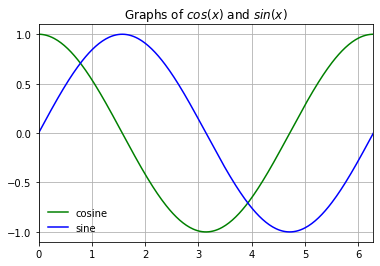
\includegraphics[keepaspectratio]{q1.png}}

    \begin{tcolorbox}[breakable, size=fbox, boxrule=1pt, pad at break*=1mm,colback=cellbackground, colframe=cellborder]
\prompt{In}{incolor}{254}{\boxspacing}
\begin{Verbatim}[commandchars=\\\{\}]
\PY{c+c1}{\PYZsh{} Here\PYZsq{}s the starting code from last time. Edit / Add code to create the plot above.}
\PY{n}{plt}\PY{o}{.}\PY{n}{plot}\PY{p}{(}\PY{n}{xs}\PY{p}{,} \PY{n}{ys}\PY{p}{)}
\PY{n}{plt}\PY{o}{.}\PY{n}{plot}\PY{p}{(}\PY{n}{xs}\PY{p}{,} \PY{n}{np}\PY{o}{.}\PY{n}{sin}\PY{p}{(}\PY{n}{xs}\PY{p}{)}\PY{p}{)}
\end{Verbatim}
\end{tcolorbox}

            \begin{tcolorbox}[breakable, size=fbox, boxrule=.5pt, pad at break*=1mm, opacityfill=0]
\prompt{Out}{outcolor}{254}{\boxspacing}
\begin{Verbatim}[commandchars=\\\{\}]
[<matplotlib.lines.Line2D at 0x13b03c8f0>]
\end{Verbatim}
\end{tcolorbox}
        
    \begin{center}
    \adjustimage{max size={0.9\linewidth}{0.9\paperheight}}{hw2_files/hw2_7_1.png}
    \end{center}
    { \hspace*{\fill} \\}
    
    \section{Part 1: Guided EDA of google play store apps
(40\%)}\label{part-1-guided-eda-of-google-play-store-apps-40}

You will be performing some basic EDA (exploratory data analysis) on
Google Play Store apps data. Feel free to edit code for clearning the
data.

    \begin{tcolorbox}[breakable, size=fbox, boxrule=1pt, pad at break*=1mm,colback=cellbackground, colframe=cellborder]
\prompt{In}{incolor}{255}{\boxspacing}
\begin{Verbatim}[commandchars=\\\{\}]
\PY{n}{google\PYZus{}play} \PY{o}{=} \PY{n}{pd}\PY{o}{.}\PY{n}{read\PYZus{}csv}\PY{p}{(}\PY{l+s+s1}{\PYZsq{}}\PY{l+s+s1}{googleplaystore.csv}\PY{l+s+s1}{\PYZsq{}}\PY{p}{)}

\PY{c+c1}{\PYZsh{} You may drop rows where Rating is NaN to avoid issues }
\PY{n}{google\PYZus{}play} \PY{o}{=} \PY{n}{google\PYZus{}play}\PY{o}{.}\PY{n}{dropna}\PY{p}{(}\PY{n}{subset}\PY{o}{=}\PY{p}{[}\PY{l+s+s1}{\PYZsq{}}\PY{l+s+s1}{Rating}\PY{l+s+s1}{\PYZsq{}}\PY{p}{]}\PY{p}{)}
\PY{n}{google\PYZus{}play}\PY{p}{[}\PY{l+s+s1}{\PYZsq{}}\PY{l+s+s1}{Rating}\PY{l+s+s1}{\PYZsq{}}\PY{p}{]} \PY{o}{=} \PY{n}{pd}\PY{o}{.}\PY{n}{to\PYZus{}numeric}\PY{p}{(}\PY{n}{google\PYZus{}play}\PY{p}{[}\PY{l+s+s1}{\PYZsq{}}\PY{l+s+s1}{Rating}\PY{l+s+s1}{\PYZsq{}}\PY{p}{]}\PY{p}{,} \PY{n}{errors}\PY{o}{=}\PY{l+s+s1}{\PYZsq{}}\PY{l+s+s1}{coerce}\PY{l+s+s1}{\PYZsq{}}\PY{p}{)}
\PY{n}{google\PYZus{}play}\PY{p}{[}\PY{l+s+s1}{\PYZsq{}}\PY{l+s+s1}{Reviews}\PY{l+s+s1}{\PYZsq{}}\PY{p}{]} \PY{o}{=} \PY{n}{pd}\PY{o}{.}\PY{n}{to\PYZus{}numeric}\PY{p}{(}\PY{n}{google\PYZus{}play}\PY{p}{[}\PY{l+s+s1}{\PYZsq{}}\PY{l+s+s1}{Reviews}\PY{l+s+s1}{\PYZsq{}}\PY{p}{]}\PY{p}{,} \PY{n}{errors}\PY{o}{=}\PY{l+s+s1}{\PYZsq{}}\PY{l+s+s1}{coerce}\PY{l+s+s1}{\PYZsq{}}\PY{p}{)}
\PY{n}{google\PYZus{}play}\PY{p}{[}\PY{l+s+s1}{\PYZsq{}}\PY{l+s+s1}{Last Updated}\PY{l+s+s1}{\PYZsq{}}\PY{p}{]} \PY{o}{=} \PY{n}{pd}\PY{o}{.}\PY{n}{to\PYZus{}datetime}\PY{p}{(}\PY{n}{google\PYZus{}play}\PY{p}{[}\PY{l+s+s1}{\PYZsq{}}\PY{l+s+s1}{Last Updated}\PY{l+s+s1}{\PYZsq{}}\PY{p}{]}\PY{p}{,} \PY{n}{errors}\PY{o}{=}\PY{l+s+s1}{\PYZsq{}}\PY{l+s+s1}{coerce}\PY{l+s+s1}{\PYZsq{}}\PY{p}{)}
\PY{n}{google\PYZus{}play} \PY{o}{=} \PY{n}{google\PYZus{}play}\PY{p}{[}\PY{n}{google\PYZus{}play}\PY{p}{[}\PY{l+s+s1}{\PYZsq{}}\PY{l+s+s1}{Category}\PY{l+s+s1}{\PYZsq{}}\PY{p}{]} \PY{o}{!=} \PY{l+s+s1}{\PYZsq{}}\PY{l+s+s1}{1.9}\PY{l+s+s1}{\PYZsq{}}\PY{p}{]}
\end{Verbatim}
\end{tcolorbox}

    \begin{tcolorbox}[breakable, size=fbox, boxrule=1pt, pad at break*=1mm,colback=cellbackground, colframe=cellborder]
\prompt{In}{incolor}{256}{\boxspacing}
\begin{Verbatim}[commandchars=\\\{\}]
\PY{n}{google\PYZus{}play}\PY{o}{.}\PY{n}{head}\PY{p}{(}\PY{p}{)}
\end{Verbatim}
\end{tcolorbox}

            \begin{tcolorbox}[breakable, size=fbox, boxrule=.5pt, pad at break*=1mm, opacityfill=0]
\prompt{Out}{outcolor}{256}{\boxspacing}
\begin{Verbatim}[commandchars=\\\{\}]
                                                 App        Category  Rating  \textbackslash{}
0     Photo Editor \& Candy Camera \& Grid \& ScrapBook  ART\_AND\_DESIGN     4.1
1                                Coloring book moana  ART\_AND\_DESIGN     3.9
2  U Launcher Lite – FREE Live Cool Themes, Hide {\ldots}  ART\_AND\_DESIGN     4.7
3                              Sketch - Draw \& Paint  ART\_AND\_DESIGN     4.5
4              Pixel Draw - Number Art Coloring Book  ART\_AND\_DESIGN     4.3

    Reviews  Size     Installs  Type Price Content Rating  \textbackslash{}
0     159.0   19M      10,000+  Free     0       Everyone
1     967.0   14M     500,000+  Free     0       Everyone
2   87510.0  8.7M   5,000,000+  Free     0       Everyone
3  215644.0   25M  50,000,000+  Free     0           Teen
4     967.0  2.8M     100,000+  Free     0       Everyone

                      Genres Last Updated         Current Ver   Android Ver
0               Art \& Design   2018-01-07               1.0.0  4.0.3 and up
1  Art \& Design;Pretend Play   2018-01-15               2.0.0  4.0.3 and up
2               Art \& Design   2018-08-01               1.2.4  4.0.3 and up
3               Art \& Design   2018-06-08  Varies with device    4.2 and up
4    Art \& Design;Creativity   2018-06-20                 1.1    4.4 and up
\end{Verbatim}
\end{tcolorbox}
        
    \subsection{Q1.1 (8\%):}\label{q1.1-8}

Explore the \texttt{google\_play} dataframe to answer the following
questions.

What is the data granularity? What time range is represented here? Write
code in the cell below to perform your exploration.

    \begin{tcolorbox}[breakable, size=fbox, boxrule=1pt, pad at break*=1mm,colback=cellbackground, colframe=cellborder]
\prompt{In}{incolor}{257}{\boxspacing}
\begin{Verbatim}[commandchars=\\\{\}]
\PY{c+c1}{\PYZsh{} The data granularity}
\PY{n}{Unique\PYZus{}google\PYZus{}play} \PY{o}{=} \PY{n}{google\PYZus{}play}\PY{o}{.}\PY{n}{pivot\PYZus{}table}\PY{p}{(}
    \PY{n}{values}\PY{o}{=}\PY{l+s+s1}{\PYZsq{}}\PY{l+s+s1}{Last Updated}\PY{l+s+s1}{\PYZsq{}}\PY{p}{,}  \PY{c+c1}{\PYZsh{} Use any column that has values for each row}
    \PY{n}{index}\PY{o}{=}\PY{l+s+s1}{\PYZsq{}}\PY{l+s+s1}{App}\PY{l+s+s1}{\PYZsq{}}\PY{p}{,}  \PY{c+c1}{\PYZsh{} Group by \PYZsq{}Category\PYZsq{} or any other column to assess granularity}
    \PY{n}{aggfunc}\PY{o}{=}\PY{l+s+s1}{\PYZsq{}}\PY{l+s+s1}{count}\PY{l+s+s1}{\PYZsq{}}  \PY{c+c1}{\PYZsh{} Count the number of entries per group}
\PY{p}{)}

\PY{c+c1}{\PYZsh{}print(Unique\PYZus{}google\PYZus{}play)}
\PY{n+nb}{print}\PY{p}{(}\PY{l+s+sa}{f}\PY{l+s+s2}{\PYZdq{}}\PY{l+s+s2}{The data granularity of unique apps: }\PY{l+s+si}{\PYZob{}}\PY{n+nb}{len}\PY{p}{(}\PY{n}{Unique\PYZus{}google\PYZus{}play}\PY{p}{)}\PY{l+s+si}{\PYZcb{}}\PY{l+s+s2}{\PYZdq{}}\PY{p}{)}
\PY{n+nb}{print}\PY{p}{(}\PY{l+s+sa}{f}\PY{l+s+s2}{\PYZdq{}}\PY{l+s+s2}{Total number of rows: }\PY{l+s+si}{\PYZob{}}\PY{n+nb}{len}\PY{p}{(}\PY{n}{google\PYZus{}play}\PY{p}{)}\PY{l+s+si}{\PYZcb{}}\PY{l+s+s2}{\PYZdq{}}\PY{p}{)}

\PY{c+c1}{\PYZsh{} The time range}
\PY{n}{min\PYZus{}date} \PY{o}{=} \PY{n}{google\PYZus{}play}\PY{p}{[}\PY{l+s+s1}{\PYZsq{}}\PY{l+s+s1}{Last Updated}\PY{l+s+s1}{\PYZsq{}}\PY{p}{]}\PY{o}{.}\PY{n}{min}\PY{p}{(}\PY{p}{)}
\PY{n}{max\PYZus{}date} \PY{o}{=} \PY{n}{google\PYZus{}play}\PY{p}{[}\PY{l+s+s1}{\PYZsq{}}\PY{l+s+s1}{Last Updated}\PY{l+s+s1}{\PYZsq{}}\PY{p}{]}\PY{o}{.}\PY{n}{max}\PY{p}{(}\PY{p}{)}

\PY{n+nb}{print}\PY{p}{(}\PY{l+s+sa}{f}\PY{l+s+s2}{\PYZdq{}}\PY{l+s+s2}{The time range is from: }\PY{l+s+si}{\PYZob{}}\PY{n}{min\PYZus{}date}\PY{l+s+si}{\PYZcb{}}\PY{l+s+s2}{ \PYZhy{} }\PY{l+s+si}{\PYZob{}}\PY{n}{max\PYZus{}date}\PY{l+s+si}{\PYZcb{}}\PY{l+s+s2}{\PYZdq{}}\PY{p}{)}
\PY{n+nb}{print}\PY{p}{(}\PY{l+s+sa}{f}\PY{l+s+s2}{\PYZdq{}}\PY{l+s+s2}{The time range represents the time period during which these apps were last updated.}\PY{l+s+s2}{\PYZdq{}}\PY{p}{)}
\end{Verbatim}
\end{tcolorbox}

    \begin{Verbatim}[commandchars=\\\{\}]
The data granularity of unique apps: 8196
Total number of rows: 9366
The time range is from: 2010-05-21 00:00:00 - 2018-08-08 00:00:00
The time range represents the time period during which these apps were last
updated.
    \end{Verbatim}

    (\emph{Your Q1.1 answer here. Double click to edit})

    \subsection{\texorpdfstring{Using \texttt{pandas} to
plot}{Using pandas to plot}}\label{using-pandas-to-plot}

\texttt{pandas} provides useful methods on dataframes. For simple plots,
we prefer to just use those methods instead of the \texttt{matplotlib}
methods since we're often working with dataframes anyway. The syntax is:

\begin{verbatim}
dataframe.plot.<plotfunc>
\end{verbatim}

Where the \texttt{\textless{}plotfunc\textgreater{}} is one of the
functions listed under \emph{Plotting} here:
https://pandas.pydata.org/pandas-docs/stable/reference/frame.html

    \begin{tcolorbox}[breakable, size=fbox, boxrule=1pt, pad at break*=1mm,colback=cellbackground, colframe=cellborder]
\prompt{In}{incolor}{258}{\boxspacing}
\begin{Verbatim}[commandchars=\\\{\}]
\PY{c+c1}{\PYZsh{} This plot shows the trend of app ratings over time}

\PY{n}{google\PYZus{}play}\PY{o}{.}\PY{n}{plot}\PY{o}{.}\PY{n}{line}\PY{p}{(}\PY{n}{x}\PY{o}{=}\PY{l+s+s1}{\PYZsq{}}\PY{l+s+s1}{Last Updated}\PY{l+s+s1}{\PYZsq{}}\PY{p}{,} \PY{n}{y}\PY{o}{=}\PY{l+s+s1}{\PYZsq{}}\PY{l+s+s1}{Reviews}\PY{l+s+s1}{\PYZsq{}}\PY{p}{)}
\end{Verbatim}
\end{tcolorbox}

            \begin{tcolorbox}[breakable, size=fbox, boxrule=.5pt, pad at break*=1mm, opacityfill=0]
\prompt{Out}{outcolor}{258}{\boxspacing}
\begin{Verbatim}[commandchars=\\\{\}]
<Axes: xlabel='Last Updated'>
\end{Verbatim}
\end{tcolorbox}
        
    \begin{center}
    \adjustimage{max size={0.9\linewidth}{0.9\paperheight}}{hw2_files/hw2_15_1.png}
    \end{center}
    { \hspace*{\fill} \\}
    
    \subsection{\texorpdfstring{\texttt{seaborn}}{seaborn}}\label{seaborn}

Now, we'll learn how to use the
\href{http://seaborn.pydata.org/index.html}{\texttt{seaborn}} Python
library. \texttt{seaborn} is built on top of \texttt{matplotlib} and
provides many helpful functions for statistical plotting that
\texttt{matplotlib} and \texttt{pandas} don't have.

Generally speaking, we'll use \texttt{seaborn} for more complex
statistical plots, \texttt{pandas} for simple plots (eg. line / scatter
plots), and \texttt{matplotlib} for plot customization.

Nearly all \texttt{seaborn} functions are designed to operate on
\texttt{pandas} dataframes. Most of these functions assume that the
dataframe is in a specific format called \emph{long-form}, where each
column of the dataframe is a particular feature and each row of the
dataframe a single datapoint.

For example, this dataframe is long-form:

\begin{verbatim}
   country year avgtemp
 1  Sweden 1994       6
 2 Denmark 1994       6
 3  Norway 1994       3
 4  Sweden 1995       5
 5 Denmark 1995       8
 6  Norway 1995      11
 7  Sweden 1996       7
 8 Denmark 1996       8
 9  Norway 1996       7
\end{verbatim}

But this dataframe of the same data is not:

\begin{verbatim}
   country avgtemp.1994 avgtemp.1995 avgtemp.1996
 1  Sweden            6            5            7
 2 Denmark            6            8            8
 3  Norway            3           11            7
\end{verbatim}

Note that the \texttt{google\_play} dataframe is long-form.

For more about long-form data, see
https://stanford.edu/\textasciitilde ejdemyr/r-tutorials/wide-and-long.
For now, just remember that we typically prefer long-form data and it
makes plotting using \texttt{seaborn} easy as well.

We can create the same plot as the \texttt{dataframe.plot} above using
the following \texttt{seaborn} function: \texttt{sns.lineplot}. Notice
that instead of calling the plot function on dataframe object, here we
pass it as a parameter to the function:

    \begin{tcolorbox}[breakable, size=fbox, boxrule=1pt, pad at break*=1mm,colback=cellbackground, colframe=cellborder]
\prompt{In}{incolor}{259}{\boxspacing}
\begin{Verbatim}[commandchars=\\\{\}]
\PY{c+c1}{\PYZsh{} You can create a plot similar to the one above using the following seaborn syntax}
\PY{c+c1}{\PYZsh{} Note that the seaborn plot is a bit different and requires some customizations (more on this later)}
\PY{n}{sns}\PY{o}{.}\PY{n}{lineplot}\PY{p}{(}\PY{n}{x}\PY{o}{=}\PY{l+s+s2}{\PYZdq{}}\PY{l+s+s2}{Last Updated}\PY{l+s+s2}{\PYZdq{}}\PY{p}{,} \PY{n}{y}\PY{o}{=}\PY{l+s+s2}{\PYZdq{}}\PY{l+s+s2}{Reviews}\PY{l+s+s2}{\PYZdq{}}\PY{p}{,} \PY{n}{data}\PY{o}{=}\PY{n}{google\PYZus{}play}\PY{p}{)}
\end{Verbatim}
\end{tcolorbox}

            \begin{tcolorbox}[breakable, size=fbox, boxrule=.5pt, pad at break*=1mm, opacityfill=0]
\prompt{Out}{outcolor}{259}{\boxspacing}
\begin{Verbatim}[commandchars=\\\{\}]
<Axes: xlabel='Last Updated', ylabel='Reviews'>
\end{Verbatim}
\end{tcolorbox}
        
    \begin{center}
    \adjustimage{max size={0.9\linewidth}{0.9\paperheight}}{hw2_files/hw2_17_1.png}
    \end{center}
    { \hspace*{\fill} \\}
    
    \subsection{Q1.2 (8\%):}\label{q1.2-8}

Use seaborn's barplot function to make a bar chart showing the average
rating for each app category over the entire \texttt{google\_play}
dataset. Here's a link to the seaborn API:

Here's a link to the seaborn API: http://seaborn.pydata.org/api.html

See if you can figure it out by reading the docs.

What trends do you notice? What do you suppose causes these trends?

Notice that \texttt{barplot} draws error bars for each category. It uses
bootstrapping to make those.

    \begin{tcolorbox}[breakable, size=fbox, boxrule=1pt, pad at break*=1mm,colback=cellbackground, colframe=cellborder]
\prompt{In}{incolor}{260}{\boxspacing}
\begin{Verbatim}[commandchars=\\\{\}]
\PY{c+c1}{\PYZsh{} Get the average rating for each app category over the entire `google\PYZus{}play` }
\PY{n}{Average\PYZus{}google\PYZus{}play} \PY{o}{=} \PY{n}{google\PYZus{}play}\PY{o}{.}\PY{n}{pivot\PYZus{}table}\PY{p}{(}
    \PY{n}{values}\PY{o}{=}\PY{l+s+s1}{\PYZsq{}}\PY{l+s+s1}{Rating}\PY{l+s+s1}{\PYZsq{}}\PY{p}{,}  \PY{c+c1}{\PYZsh{} Use any column that has values for each row}
    \PY{n}{index}\PY{o}{=}\PY{l+s+s1}{\PYZsq{}}\PY{l+s+s1}{Category}\PY{l+s+s1}{\PYZsq{}}\PY{p}{,}  \PY{c+c1}{\PYZsh{} Group by \PYZsq{}Category\PYZsq{} or any other column to assess granularity}
    \PY{n}{aggfunc}\PY{o}{=}\PY{l+s+s1}{\PYZsq{}}\PY{l+s+s1}{mean}\PY{l+s+s1}{\PYZsq{}}  \PY{c+c1}{\PYZsh{} Count the number of entries per group}
\PY{p}{)}
\PY{n}{sns}\PY{o}{.}\PY{n}{barplot}\PY{p}{(}\PY{n}{Average\PYZus{}google\PYZus{}play}\PY{p}{,} \PY{n}{x}\PY{o}{=}\PY{l+s+s2}{\PYZdq{}}\PY{l+s+s2}{Rating}\PY{l+s+s2}{\PYZdq{}}\PY{p}{,} \PY{n}{y}\PY{o}{=}\PY{l+s+s2}{\PYZdq{}}\PY{l+s+s2}{Category}\PY{l+s+s2}{\PYZdq{}}\PY{p}{,} \PY{n}{errorbar}\PY{o}{=}\PY{k+kc}{None}\PY{p}{)}
\PY{n+nb}{print}\PY{p}{(}\PY{l+s+sa}{f}\PY{l+s+s2}{\PYZdq{}}\PY{l+s+s2}{The most app categories have high average ratings, generally around 4.0 to 4.5.}\PY{l+s+s2}{\PYZdq{}}\PY{p}{)}
\PY{n+nb}{print}\PY{p}{(}\PY{l+s+sa}{f}\PY{l+s+s2}{\PYZdq{}}\PY{l+s+s2}{This trend maybe caused by the frequencey od update to improve the quality of app.}\PY{l+s+s2}{\PYZdq{}}\PY{p}{)}
\end{Verbatim}
\end{tcolorbox}

    \begin{Verbatim}[commandchars=\\\{\}]
The most app categories have high average ratings, generally around 4.0 to 4.5.
This trend maybe caused by the frequencey od update to improve the quality of
app.
    \end{Verbatim}

    \begin{center}
    \adjustimage{max size={0.9\linewidth}{0.9\paperheight}}{hw2_files/hw2_19_1.png}
    \end{center}
    { \hspace*{\fill} \\}
    
    (Your Q1.2 answer here)

The most app categories have high average ratings, generally around 4.0
to 4.5. This trend maybe caused by the frequencey od update to improve
the quality of app.

    \subsection{Q1.3 (8\%):}\label{q1.3-8}

Now for a fancier plot that \texttt{seaborn} makes really easy to
produce.

Use the \texttt{displot} function to plot a histogram of all the ratings
in the \texttt{google\_play} dataset. Can you fit a curve to the
histogram of the data using \texttt{seaborn}? You just need to tune
\texttt{kde} and \texttt{stat} paramaters to the \texttt{displot}
function. Fancy!

    \begin{tcolorbox}[breakable, size=fbox, boxrule=1pt, pad at break*=1mm,colback=cellbackground, colframe=cellborder]
\prompt{In}{incolor}{261}{\boxspacing}
\begin{Verbatim}[commandchars=\\\{\}]
\PY{c+c1}{\PYZsh{} Plot a histogram of all the ratings in the `google\PYZus{}play` dataset}
\PY{n}{sns}\PY{o}{.}\PY{n}{displot}\PY{p}{(}\PY{n}{data}\PY{o}{=}\PY{n}{google\PYZus{}play}\PY{p}{,} \PY{n}{x}\PY{o}{=}\PY{l+s+s2}{\PYZdq{}}\PY{l+s+s2}{Rating}\PY{l+s+s2}{\PYZdq{}}\PY{p}{)}

\PY{c+c1}{\PYZsh{} fit a curve to the histogram of the data}
\PY{n}{sns}\PY{o}{.}\PY{n}{displot}\PY{p}{(}\PY{n}{data}\PY{o}{=}\PY{n}{google\PYZus{}play}\PY{p}{,} \PY{n}{x}\PY{o}{=}\PY{l+s+s2}{\PYZdq{}}\PY{l+s+s2}{Rating}\PY{l+s+s2}{\PYZdq{}}\PY{p}{,}\PY{n}{kde}\PY{o}{=}\PY{k+kc}{True}\PY{p}{,}\PY{n}{stat}\PY{o}{=}\PY{l+s+s2}{\PYZdq{}}\PY{l+s+s2}{density}\PY{l+s+s2}{\PYZdq{}}\PY{p}{)}
\end{Verbatim}
\end{tcolorbox}

            \begin{tcolorbox}[breakable, size=fbox, boxrule=.5pt, pad at break*=1mm, opacityfill=0]
\prompt{Out}{outcolor}{261}{\boxspacing}
\begin{Verbatim}[commandchars=\\\{\}]
<seaborn.axisgrid.FacetGrid at 0x13259f500>
\end{Verbatim}
\end{tcolorbox}
        
    \begin{center}
    \adjustimage{max size={0.9\linewidth}{0.9\paperheight}}{hw2_files/hw2_22_1.png}
    \end{center}
    { \hspace*{\fill} \\}
    
    \begin{center}
    \adjustimage{max size={0.9\linewidth}{0.9\paperheight}}{hw2_files/hw2_22_2.png}
    \end{center}
    { \hspace*{\fill} \\}
    
    \subsection{Q1.4 (8\%):}\label{q1.4-8}

Use \texttt{seaborn} to make side-by-side boxplots of the number of
reviews and app size for the apps in the \texttt{google\_play} dataset.
The \texttt{boxplot} function will plot all the columns of the dataframe
you pass in.

Note that, you may need to pre-process the `Size' column for numeric
analysis. Hint: you may want to convert kb to mb.

Once you make the plot, you'll notice that there are many outliers that
make the plot hard to see. To mitigate this, change the y-scale to be
logarithmic.

That's a plot customization so you'll use \texttt{matplotlib}. The
\texttt{boxplot} function returns a \texttt{matplotlib} Axes object
which represents a single plot and has a \texttt{set\_yscale} function.

The result (after customization) should look like:

\pandocbounded{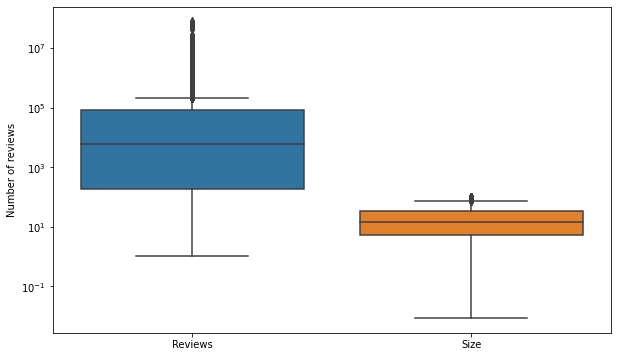
\includegraphics[keepaspectratio]{q1-4.png}}

Revisiting Q1.1 on data granularity, what is more suitable text for
\texttt{ylabel} here than \texttt{Number\ of\ reviews}?

    \begin{tcolorbox}[breakable, size=fbox, boxrule=1pt, pad at break*=1mm,colback=cellbackground, colframe=cellborder]
\prompt{In}{incolor}{262}{\boxspacing}
\begin{Verbatim}[commandchars=\\\{\}]
\PY{c+c1}{\PYZsh{} pre\PYZhy{}process the \PYZsq{}Size\PYZsq{} column for numeric analysis}
\PY{n}{google\PYZus{}play}\PY{p}{[}\PY{l+s+s1}{\PYZsq{}}\PY{l+s+s1}{Size}\PY{l+s+s1}{\PYZsq{}}\PY{p}{]} \PY{o}{=} \PY{n}{google\PYZus{}play}\PY{p}{[}\PY{l+s+s1}{\PYZsq{}}\PY{l+s+s1}{Size}\PY{l+s+s1}{\PYZsq{}}\PY{p}{]}\PY{o}{.}\PY{n}{astype}\PY{p}{(}\PY{n+nb}{str}\PY{p}{)}
\PY{n}{google\PYZus{}play}\PY{p}{[}\PY{l+s+s1}{\PYZsq{}}\PY{l+s+s1}{Size}\PY{l+s+s1}{\PYZsq{}}\PY{p}{]} \PY{o}{=} \PY{n}{google\PYZus{}play}\PY{p}{[}\PY{l+s+s1}{\PYZsq{}}\PY{l+s+s1}{Size}\PY{l+s+s1}{\PYZsq{}}\PY{p}{]}\PY{o}{.}\PY{n}{replace}\PY{p}{(}\PY{l+s+s1}{\PYZsq{}}\PY{l+s+s1}{Varies with device}\PY{l+s+s1}{\PYZsq{}}\PY{p}{,} \PY{k+kc}{None}\PY{p}{)}

\PY{n}{sizes\PYZus{}mb} \PY{o}{=} \PY{p}{[}\PY{p}{]}
\PY{k}{for} \PY{n}{x} \PY{o+ow}{in} \PY{n}{google\PYZus{}play}\PY{p}{[}\PY{l+s+s1}{\PYZsq{}}\PY{l+s+s1}{Size}\PY{l+s+s1}{\PYZsq{}}\PY{p}{]}\PY{p}{:}
    \PY{k}{if} \PY{l+s+s1}{\PYZsq{}}\PY{l+s+s1}{M}\PY{l+s+s1}{\PYZsq{}} \PY{o+ow}{in} \PY{n+nb}{str}\PY{p}{(}\PY{n}{x}\PY{p}{)}\PY{p}{:}
        \PY{n}{sizes\PYZus{}mb}\PY{o}{.}\PY{n}{append}\PY{p}{(}\PY{n+nb}{float}\PY{p}{(}\PY{n}{x}\PY{o}{.}\PY{n}{replace}\PY{p}{(}\PY{l+s+s1}{\PYZsq{}}\PY{l+s+s1}{M}\PY{l+s+s1}{\PYZsq{}}\PY{p}{,} \PY{l+s+s1}{\PYZsq{}}\PY{l+s+s1}{\PYZsq{}}\PY{p}{)}\PY{p}{)}\PY{p}{)}
    \PY{k}{elif} \PY{l+s+s1}{\PYZsq{}}\PY{l+s+s1}{K}\PY{l+s+s1}{\PYZsq{}} \PY{o+ow}{in} \PY{n+nb}{str}\PY{p}{(}\PY{n}{x}\PY{p}{)}\PY{p}{:}
        \PY{n}{sizes\PYZus{}mb}\PY{o}{.}\PY{n}{append}\PY{p}{(}\PY{n+nb}{float}\PY{p}{(}\PY{n}{x}\PY{o}{.}\PY{n}{replace}\PY{p}{(}\PY{l+s+s1}{\PYZsq{}}\PY{l+s+s1}{M}\PY{l+s+s1}{\PYZsq{}}\PY{p}{,} \PY{l+s+s1}{\PYZsq{}}\PY{l+s+s1}{\PYZsq{}}\PY{p}{)}\PY{p}{)}\PY{o}{/}\PY{o}{/}\PY{l+m+mi}{1024}\PY{p}{)}
    \PY{k}{else}\PY{p}{:}
        \PY{n}{sizes\PYZus{}mb}\PY{o}{.}\PY{n}{append}\PY{p}{(}\PY{k+kc}{None}\PY{p}{)}

\PY{n}{google\PYZus{}play}\PY{p}{[}\PY{l+s+s1}{\PYZsq{}}\PY{l+s+s1}{Size\PYZus{}MB}\PY{l+s+s1}{\PYZsq{}}\PY{p}{]} \PY{o}{=} \PY{n}{pd}\PY{o}{.}\PY{n}{to\PYZus{}numeric}\PY{p}{(}\PY{n}{sizes\PYZus{}mb}\PY{p}{,} \PY{n}{errors}\PY{o}{=}\PY{l+s+s1}{\PYZsq{}}\PY{l+s+s1}{coerce}\PY{l+s+s1}{\PYZsq{}}\PY{p}{)}

\PY{c+c1}{\PYZsh{} Creating side\PYZhy{}by\PYZhy{}side boxplots for Review and Size}
\PY{n}{plt}\PY{o}{.}\PY{n}{figure}\PY{p}{(}\PY{n}{figsize}\PY{o}{=}\PY{p}{(}\PY{l+m+mi}{10}\PY{p}{,} \PY{l+m+mi}{6}\PY{p}{)}\PY{p}{)}
\PY{n}{sns}\PY{o}{.}\PY{n}{boxplot}\PY{p}{(}\PY{n}{data}\PY{o}{=}\PY{n}{google\PYZus{}play}\PY{p}{[}\PY{p}{[}\PY{l+s+s1}{\PYZsq{}}\PY{l+s+s1}{Reviews}\PY{l+s+s1}{\PYZsq{}}\PY{p}{,} \PY{l+s+s1}{\PYZsq{}}\PY{l+s+s1}{Size\PYZus{}MB}\PY{l+s+s1}{\PYZsq{}}\PY{p}{]}\PY{p}{]}\PY{p}{)}
\PY{c+c1}{\PYZsh{} change the y\PYZhy{}scale to be logarithmic.}
\PY{n}{plt}\PY{o}{.}\PY{n}{yscale}\PY{p}{(}\PY{l+s+s1}{\PYZsq{}}\PY{l+s+s1}{log}\PY{l+s+s1}{\PYZsq{}}\PY{p}{)}
\PY{n}{plt}\PY{o}{.}\PY{n}{show}\PY{p}{(}\PY{p}{)}
\end{Verbatim}
\end{tcolorbox}

    \begin{center}
    \adjustimage{max size={0.9\linewidth}{0.9\paperheight}}{hw2_files/hw2_24_0.png}
    \end{center}
    { \hspace*{\fill} \\}
    
    \subsection{Q1.5 (8\%):}\label{q1.5-8}

Let's take a closer look at the number of reviews vs.~rating.

Use the \texttt{lmplot} function to make a scatterplot. Put the number
of reviews on the x-axis and the rating on the y-axis. Each point should
correspond to a single row in your \texttt{google\_play} dataframe.
Notice that \texttt{seaborn} automatically fits a line of best fit to
the plot. Does that line seem to be relevant?

You should note that \texttt{lmplot} allows you to pass in
\texttt{fit\_reg=False} to avoid plotting lines of best fit when you
feel they are unnecessary or misleading.

There seem to be two main groups in the scatterplot. Let's see if we can
separate them out. Use \texttt{lmplot} to make the scatterplot again.
This time, use the \texttt{hue} parameter to color points for free apps
differently from paid apps.

Note that, you may need to pre-process the `Type' column, only keep rows
where `Type' is ``Free'' or ``Paid''.

You should get something that looks like:

\pandocbounded{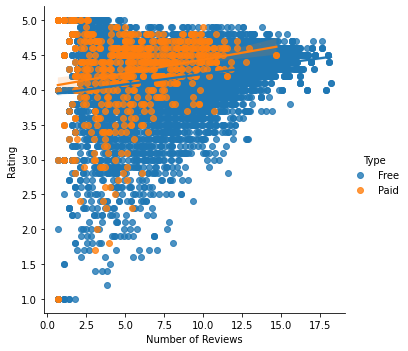
\includegraphics[keepaspectratio]{q1-5.png}}

    \begin{tcolorbox}[breakable, size=fbox, boxrule=1pt, pad at break*=1mm,colback=cellbackground, colframe=cellborder]
\prompt{In}{incolor}{263}{\boxspacing}
\begin{Verbatim}[commandchars=\\\{\}]
\PY{c+c1}{\PYZsh{} Hint: Use log number of reviews makes it easier to observe the app data}
\PY{c+c1}{\PYZsh{} so you may want to use \PYZsq{}Log\PYZus{}Reviews\PYZsq{} for this question}
\PY{n}{google\PYZus{}play}\PY{p}{[}\PY{l+s+s1}{\PYZsq{}}\PY{l+s+s1}{Log\PYZus{}Reviews}\PY{l+s+s1}{\PYZsq{}}\PY{p}{]} \PY{o}{=} \PY{n}{np}\PY{o}{.}\PY{n}{log1p}\PY{p}{(}\PY{n}{google\PYZus{}play}\PY{p}{[}\PY{l+s+s1}{\PYZsq{}}\PY{l+s+s1}{Reviews}\PY{l+s+s1}{\PYZsq{}}\PY{p}{]}\PY{p}{)}
\end{Verbatim}
\end{tcolorbox}

    \begin{tcolorbox}[breakable, size=fbox, boxrule=1pt, pad at break*=1mm,colback=cellbackground, colframe=cellborder]
\prompt{In}{incolor}{264}{\boxspacing}
\begin{Verbatim}[commandchars=\\\{\}]
\PY{c+c1}{\PYZsh{} Scatterplot with plotting lines}
\PY{n}{sns}\PY{o}{.}\PY{n}{lmplot}\PY{p}{(}\PY{n}{data}\PY{o}{=}\PY{n}{google\PYZus{}play}\PY{p}{,} \PY{n}{x}\PY{o}{=}\PY{l+s+s2}{\PYZdq{}}\PY{l+s+s2}{Log\PYZus{}Reviews}\PY{l+s+s2}{\PYZdq{}}\PY{p}{,} \PY{n}{y}\PY{o}{=}\PY{l+s+s2}{\PYZdq{}}\PY{l+s+s2}{Rating}\PY{l+s+s2}{\PYZdq{}}\PY{p}{)}
\PY{c+c1}{\PYZsh{} Scatterplot without plotting lines}
\PY{n}{sns}\PY{o}{.}\PY{n}{lmplot}\PY{p}{(}\PY{n}{data}\PY{o}{=}\PY{n}{google\PYZus{}play}\PY{p}{,} \PY{n}{x}\PY{o}{=}\PY{l+s+s2}{\PYZdq{}}\PY{l+s+s2}{Log\PYZus{}Reviews}\PY{l+s+s2}{\PYZdq{}}\PY{p}{,} \PY{n}{y}\PY{o}{=}\PY{l+s+s2}{\PYZdq{}}\PY{l+s+s2}{Rating}\PY{l+s+s2}{\PYZdq{}}\PY{p}{,}\PY{n}{fit\PYZus{}reg}\PY{o}{=}\PY{k+kc}{False}\PY{p}{)}
\PY{c+c1}{\PYZsh{} Scatterplot with different color}
\PY{n}{sns}\PY{o}{.}\PY{n}{lmplot}\PY{p}{(}\PY{n}{data}\PY{o}{=}\PY{n}{google\PYZus{}play}\PY{p}{,} \PY{n}{x}\PY{o}{=}\PY{l+s+s2}{\PYZdq{}}\PY{l+s+s2}{Log\PYZus{}Reviews}\PY{l+s+s2}{\PYZdq{}}\PY{p}{,} \PY{n}{y}\PY{o}{=}\PY{l+s+s2}{\PYZdq{}}\PY{l+s+s2}{Rating}\PY{l+s+s2}{\PYZdq{}}\PY{p}{,}\PY{n}{hue}\PY{o}{=}\PY{l+s+s2}{\PYZdq{}}\PY{l+s+s2}{Type}\PY{l+s+s2}{\PYZdq{}}\PY{p}{)}

\PY{n+nb}{print}\PY{p}{(}\PY{l+s+sa}{f}\PY{l+s+s2}{\PYZdq{}}\PY{l+s+s2}{Yes, I think this line is relevant. the line of best fit shows a trend where the rating increases with the number of reviews for both free and paid apps. }\PY{l+s+s2}{\PYZdq{}}\PY{p}{)}
\end{Verbatim}
\end{tcolorbox}

    \begin{Verbatim}[commandchars=\\\{\}]
Yes, I think this line is relevant. the line of best fit shows a trend where the
rating increases with the number of reviews for both free and paid apps.
    \end{Verbatim}

    \begin{center}
    \adjustimage{max size={0.9\linewidth}{0.9\paperheight}}{hw2_files/hw2_27_1.png}
    \end{center}
    { \hspace*{\fill} \\}
    
    \begin{center}
    \adjustimage{max size={0.9\linewidth}{0.9\paperheight}}{hw2_files/hw2_27_2.png}
    \end{center}
    { \hspace*{\fill} \\}
    
    \begin{center}
    \adjustimage{max size={0.9\linewidth}{0.9\paperheight}}{hw2_files/hw2_27_3.png}
    \end{center}
    { \hspace*{\fill} \\}
    
    \subsection{Want to learn more?}\label{want-to-learn-more}

We recommend checking out the \texttt{seaborn} tutorials on your own
time. http://seaborn.pydata.org/tutorial.html

The \texttt{matplotlib} tutorial we linked in Question 1 is also a great
refresher on common \texttt{matplotlib} functions:
https://www.labri.fr/perso/nrougier/teaching/matplotlib/

Here's a great blog post about the differences between Python's
visualization libraries:
https://dansaber.wordpress.com/2016/10/02/a-dramatic-tour-through-pythons-data-visualization-landscape-including-ggplot-and-altair/

\section{Part 2: Self-directed EDA of Religious composition of the
world's migrants
(40\%)}\label{part-2-self-directed-eda-of-religious-composition-of-the-worlds-migrants-40}

The last part is intentionally more open-ended and will be graded on the
completeness of the plot(s) produced and the insights you gain from
them. The goal here is for you to thoroughly explore a dataset on the
religious breakdown of immigrants to, and emigrants from, countries and
regions of the world.

\emph{Question 2.0} is asking you to look at a given visualization and
reverse engineer the code that created it. \emph{Question 2.1} is about
\emph{data exploration visualization} while the other questions are
about \emph{data presentation visualization}. Report your three most
significant findings (\emph{Q2.2, Q2.3, and Q2.4}). Each finding should
have a \emph{visualization headline} which highlights the main takeaway
in 5-15 words, an informative visualization that supports your finding
and a \emph{visualization description}, 100-150 words per finding
explaining your assumptions and what you have found. For example, the
visualization headline could be ``?'' with the following bar plot
visualization:

The survey data that you will analyze was collected by Pew Research. In
order to access it, you need to create an account and download it from
\href{https://www.pewresearch.org/dataset/dataset-religious-composition-of-the-worlds-migrants-1990-2020/}{here}
(click on ``Download Dataset'' in upper right corner). The file you will
work with is \texttt{Incoming\ and\ Outgoing\ Migrant\ Counts.csv}.

Be sure to consider transformations, subsets, correlations, reference
markers, and lines/curves-of-best-fit (as covered in Chapter 6 of PTDS)
to reveal the relationship that you are wanting to learn more about.
Also be sure to make plots that are appropriate for the variable types.
For completeness, be explicit about any assumptions you make in your
analysis. An exemplary plot will have:

\begin{itemize}
\tightlist
\item
  A title
\item
  Labelled and appropriately scaled axes
\item
  A legend, if applicable
\item
  A carefully selected color scheme
\item
  A main point, accentuated through design choices
\end{itemize}

\subsection{Q2.0 (10\%): Reverse
Engineer}\label{q2.0-10-reverse-engineer}

Your first step is to load the data from
\texttt{Incoming\ and\ Outgoing\ Migrant\ Counts.csv}, and understand
what is stored in it. Your assignment is to replicate the bar plot
visualization shown above. Notice the labels on x and y axes as well as
the legend of the plot to determine the information needed to construct
the plot.

    \begin{tcolorbox}[breakable, size=fbox, boxrule=1pt, pad at break*=1mm,colback=cellbackground, colframe=cellborder]
\prompt{In}{incolor}{265}{\boxspacing}
\begin{Verbatim}[commandchars=\\\{\}]
\PY{c+c1}{\PYZsh{}HINTS}
\PY{c+c1}{\PYZsh{} 1) Read your dataframe with pandas}
\PY{n}{Incoming\PYZus{}and\PYZus{}Outgoing\PYZus{}Migrant\PYZus{}Count}\PY{o}{=} \PY{n}{pd}\PY{o}{.}\PY{n}{read\PYZus{}csv}\PY{p}{(}\PY{l+s+s1}{\PYZsq{}}\PY{l+s+s1}{Incoming and Outgoing Migrant Counts.csv}\PY{l+s+s1}{\PYZsq{}}\PY{p}{)}

\PY{c+c1}{\PYZsh{} 2) Identify what colums are used for plot above}
\PY{c+c1}{\PYZsh{} 3) Filter required rows and columns necessary for plotting above figure}
\PY{c+c1}{\PYZsh{} 4) Pre\PYZhy{}process the rows may cause issues}
\PY{c+c1}{\PYZsh{} Hint: there are some values in \PYZsq{}Count\PYZsq{} is \PYZlt{} 10,000, you can change them to 10,000.}
\PY{n}{Incoming\PYZus{}and\PYZus{}Outgoing\PYZus{}Migrant\PYZus{}Count}\PY{p}{[}\PY{l+s+s1}{\PYZsq{}}\PY{l+s+s1}{Count}\PY{l+s+s1}{\PYZsq{}}\PY{p}{]} \PY{o}{=} \PY{n}{Incoming\PYZus{}and\PYZus{}Outgoing\PYZus{}Migrant\PYZus{}Count}\PY{p}{[}\PY{l+s+s1}{\PYZsq{}}\PY{l+s+s1}{Count}\PY{l+s+s1}{\PYZsq{}}\PY{p}{]}\PY{o}{.}\PY{n}{replace}\PY{p}{(}\PY{l+s+s1}{\PYZsq{}}\PY{l+s+s1}{\PYZlt{} 10,000}\PY{l+s+s1}{\PYZsq{}}\PY{p}{,} \PY{l+s+s1}{\PYZsq{}}\PY{l+s+s1}{10000}\PY{l+s+s1}{\PYZsq{}}\PY{p}{)}
\PY{n}{Incoming\PYZus{}and\PYZus{}Outgoing\PYZus{}Migrant\PYZus{}Count}\PY{p}{[}\PY{l+s+s1}{\PYZsq{}}\PY{l+s+s1}{Count}\PY{l+s+s1}{\PYZsq{}}\PY{p}{]} \PY{o}{=} \PY{n}{Incoming\PYZus{}and\PYZus{}Outgoing\PYZus{}Migrant\PYZus{}Count}\PY{p}{[}\PY{l+s+s1}{\PYZsq{}}\PY{l+s+s1}{Count}\PY{l+s+s1}{\PYZsq{}}\PY{p}{]}\PY{o}{.}\PY{n}{str}\PY{o}{.}\PY{n}{replace}\PY{p}{(}\PY{l+s+s1}{\PYZsq{}}\PY{l+s+s1}{,}\PY{l+s+s1}{\PYZsq{}}\PY{p}{,} \PY{l+s+s1}{\PYZsq{}}\PY{l+s+s1}{\PYZsq{}}\PY{p}{)}  \PY{c+c1}{\PYZsh{} 移除逗号}
\PY{n}{Incoming\PYZus{}and\PYZus{}Outgoing\PYZus{}Migrant\PYZus{}Count}\PY{p}{[}\PY{l+s+s1}{\PYZsq{}}\PY{l+s+s1}{Count}\PY{l+s+s1}{\PYZsq{}}\PY{p}{]} \PY{o}{=} \PY{n}{pd}\PY{o}{.}\PY{n}{to\PYZus{}numeric}\PY{p}{(}\PY{n}{Incoming\PYZus{}and\PYZus{}Outgoing\PYZus{}Migrant\PYZus{}Count}\PY{p}{[}\PY{l+s+s1}{\PYZsq{}}\PY{l+s+s1}{Count}\PY{l+s+s1}{\PYZsq{}}\PY{p}{]}\PY{p}{,} \PY{n}{errors}\PY{o}{=}\PY{l+s+s1}{\PYZsq{}}\PY{l+s+s1}{coerce}\PY{l+s+s1}{\PYZsq{}}\PY{p}{)}
\PY{n}{Incoming\PYZus{}and\PYZus{}Outgoing\PYZus{}Migrant\PYZus{}Count}\PY{p}{[}\PY{l+s+s1}{\PYZsq{}}\PY{l+s+s1}{Percent}\PY{l+s+s1}{\PYZsq{}}\PY{p}{]} \PY{o}{=} \PY{n}{pd}\PY{o}{.}\PY{n}{to\PYZus{}numeric}\PY{p}{(}\PY{n}{Incoming\PYZus{}and\PYZus{}Outgoing\PYZus{}Migrant\PYZus{}Count}\PY{p}{[}\PY{l+s+s1}{\PYZsq{}}\PY{l+s+s1}{Percent}\PY{l+s+s1}{\PYZsq{}}\PY{p}{]}\PY{p}{,} \PY{n}{errors}\PY{o}{=}\PY{l+s+s1}{\PYZsq{}}\PY{l+s+s1}{coerce}\PY{l+s+s1}{\PYZsq{}}\PY{p}{)}
\PY{n}{Incoming\PYZus{}and\PYZus{}Outgoing\PYZus{}Migrant\PYZus{}Count}\PY{p}{[}\PY{l+s+s1}{\PYZsq{}}\PY{l+s+s1}{level}\PY{l+s+s1}{\PYZsq{}}\PY{p}{]} \PY{o}{=} \PY{n}{pd}\PY{o}{.}\PY{n}{to\PYZus{}numeric}\PY{p}{(}\PY{n}{Incoming\PYZus{}and\PYZus{}Outgoing\PYZus{}Migrant\PYZus{}Count}\PY{p}{[}\PY{l+s+s1}{\PYZsq{}}\PY{l+s+s1}{level}\PY{l+s+s1}{\PYZsq{}}\PY{p}{]}\PY{p}{,} \PY{n}{errors}\PY{o}{=}\PY{l+s+s1}{\PYZsq{}}\PY{l+s+s1}{coerce}\PY{l+s+s1}{\PYZsq{}}\PY{p}{)}
\PY{n}{Incoming\PYZus{}and\PYZus{}Outgoing\PYZus{}Migrant\PYZus{}Count} \PY{o}{=} \PY{n}{Incoming\PYZus{}and\PYZus{}Outgoing\PYZus{}Migrant\PYZus{}Count}\PY{p}{[}\PY{n}{Incoming\PYZus{}and\PYZus{}Outgoing\PYZus{}Migrant\PYZus{}Count}\PY{p}{[}\PY{l+s+s1}{\PYZsq{}}\PY{l+s+s1}{Religion}\PY{l+s+s1}{\PYZsq{}}\PY{p}{]} \PY{o}{!=} \PY{l+s+s1}{\PYZsq{}}\PY{l+s+s1}{All}\PY{l+s+s1}{\PYZsq{}}\PY{p}{]}
\PY{n}{Incoming\PYZus{}and\PYZus{}Outgoing\PYZus{}Migrant\PYZus{}Count}\PY{o}{.}\PY{n}{head}\PY{p}{(}\PY{p}{)}

\PY{c+c1}{\PYZsh{} 4) Use pandas aggregation to group by Region and Religion and sum the migrant counts}
\PY{n}{grouped\PYZus{}data} \PY{o}{=} \PY{n}{Incoming\PYZus{}and\PYZus{}Outgoing\PYZus{}Migrant\PYZus{}Count}\PY{o}{.}\PY{n}{groupby}\PY{p}{(}\PY{p}{[}\PY{l+s+s1}{\PYZsq{}}\PY{l+s+s1}{Region}\PY{l+s+s1}{\PYZsq{}}\PY{p}{,} \PY{l+s+s1}{\PYZsq{}}\PY{l+s+s1}{Religion}\PY{l+s+s1}{\PYZsq{}}\PY{p}{]}\PY{p}{,} \PY{n}{as\PYZus{}index}\PY{o}{=}\PY{k+kc}{False}\PY{p}{)}\PY{p}{[}\PY{l+s+s1}{\PYZsq{}}\PY{l+s+s1}{Count}\PY{l+s+s1}{\PYZsq{}}\PY{p}{]}\PY{o}{.}\PY{n}{sum}\PY{p}{(}\PY{p}{)}
\PY{n+nb}{print}\PY{p}{(}\PY{n}{grouped\PYZus{}data}\PY{p}{)}

\PY{c+c1}{\PYZsh{} 5) Use seaborn barplot to plot the figure above. Customize with color palette=\PYZsq{}viridis\PYZsq{}}
\PY{n}{sns}\PY{o}{.}\PY{n}{barplot}\PY{p}{(}\PY{n}{grouped\PYZus{}data}\PY{p}{,} \PY{n}{x}\PY{o}{=}\PY{l+s+s2}{\PYZdq{}}\PY{l+s+s2}{Region}\PY{l+s+s2}{\PYZdq{}}\PY{p}{,} \PY{n}{y}\PY{o}{=}\PY{l+s+s2}{\PYZdq{}}\PY{l+s+s2}{Count}\PY{l+s+s2}{\PYZdq{}}\PY{p}{,} \PY{n}{hue}\PY{o}{=}\PY{l+s+s2}{\PYZdq{}}\PY{l+s+s2}{Religion}\PY{l+s+s2}{\PYZdq{}}\PY{p}{,}\PY{n}{palette}\PY{o}{=}\PY{l+s+s1}{\PYZsq{}}\PY{l+s+s1}{viridis}\PY{l+s+s1}{\PYZsq{}}\PY{p}{)}

\PY{c+c1}{\PYZsh{} 6) Add descriptive xlabel, ylabel, and title}
\PY{n}{plt}\PY{o}{.}\PY{n}{title}\PY{p}{(}\PY{l+s+s1}{\PYZsq{}}\PY{l+s+s1}{Migrant Counts by Region and Religion}\PY{l+s+s1}{\PYZsq{}}\PY{p}{)} 
\PY{n}{plt}\PY{o}{.}\PY{n}{xlabel}\PY{p}{(}\PY{l+s+s1}{\PYZsq{}}\PY{l+s+s1}{Region}\PY{l+s+s1}{\PYZsq{}}\PY{p}{)}
\PY{n}{plt}\PY{o}{.}\PY{n}{ylabel}\PY{p}{(}\PY{l+s+s1}{\PYZsq{}}\PY{l+s+s1}{Total Migrant Count in millions}\PY{l+s+s1}{\PYZsq{}}\PY{p}{)}
\PY{c+c1}{\PYZsh{} 7) change the y\PYZhy{}scale to be logarithmic for better visualization}
\PY{n}{plt}\PY{o}{.}\PY{n}{yscale}\PY{p}{(}\PY{l+s+s1}{\PYZsq{}}\PY{l+s+s1}{log}\PY{l+s+s1}{\PYZsq{}}\PY{p}{)}  
\PY{n}{plt}\PY{o}{.}\PY{n}{xticks}\PY{p}{(}\PY{n}{rotation}\PY{o}{=}\PY{l+m+mi}{45}\PY{p}{)}
\PY{c+c1}{\PYZsh{} 8) Customize legend if necessary}
\PY{n}{plt}\PY{o}{.}\PY{n}{legend}\PY{p}{(}\PY{n}{title}\PY{o}{=}\PY{l+s+s1}{\PYZsq{}}\PY{l+s+s1}{Religion}\PY{l+s+s1}{\PYZsq{}}\PY{p}{)}
\PY{n}{plt}\PY{o}{.}\PY{n}{show}\PY{p}{(}\PY{p}{)}
\end{Verbatim}
\end{tcolorbox}

    \begin{Verbatim}[commandchars=\\\{\}]
                      Region      Religion       Count
0               Asia-Pacific      Buddhist   181130000
1               Asia-Pacific     Christian   383400000
2               Asia-Pacific         Hindu   235830000
3               Asia-Pacific           Jew    11810000
4               Asia-Pacific        Muslim   573790000
5               Asia-Pacific         Other    48520000
6               Asia-Pacific  Unaffiliated   235450000
7                     Europe      Buddhist    19880000
8                     Europe     Christian  1055010000
9                     Europe         Hindu    18310000
10                    Europe           Jew    28780000
11                    Europe        Muslim   211270000
12                    Europe         Other    21040000
13                    Europe  Unaffiliated   367530000
14                    Global      Buddhist   106620000
15                    Global     Christian  1364800000
16                    Global         Hindu   149780000
17                    Global           Jew    37240000
18                    Global        Muslim   749880000
19                    Global         Other    51720000
20                    Global  Unaffiliated   396660000
21   Latin America-Caribbean      Buddhist     7990000
22   Latin America-Caribbean     Christian   471240000
23   Latin America-Caribbean         Hindu     7800000
24   Latin America-Caribbean           Jew     9240000
25   Latin America-Caribbean        Muslim     7960000
26   Latin America-Caribbean         Other    12320000
27   Latin America-Caribbean  Unaffiliated    62490000
28  Middle East-North Africa      Buddhist     3210000
29  Middle East-North Africa     Christian    65150000
30  Middle East-North Africa         Hindu    26170000
31  Middle East-North Africa           Jew    33410000
32  Middle East-North Africa        Muslim   485990000
33  Middle East-North Africa         Other     4440000
34  Middle East-North Africa  Unaffiliated    19050000
35             North America      Buddhist    18040000
36             North America     Christian   473130000
37             North America         Hindu    26540000
38             North America           Jew     8860000
39             North America        Muslim    41550000
40             North America         Other    11020000
41             North America  Unaffiliated    98860000
42        Sub-Saharan Africa      Buddhist     7360000
43        Sub-Saharan Africa     Christian   286710000
44        Sub-Saharan Africa         Hindu     9980000
45        Sub-Saharan Africa           Jew     8340000
46        Sub-Saharan Africa        Muslim   191910000
47        Sub-Saharan Africa         Other    25560000
48        Sub-Saharan Africa  Unaffiliated    21660000
    \end{Verbatim}

    \begin{center}
    \adjustimage{max size={0.9\linewidth}{0.9\paperheight}}{hw2_files/hw2_29_1.png}
    \end{center}
    { \hspace*{\fill} \\}
    
    \subsection{Q2.1 (5\%): Initial
exploration}\label{q2.1-5-initial-exploration}

Run descriptive statistics on the data by considering the EDA key data
properties we covered in class. Write a 100-150 word description of your
findings. Based on these statistics or other ideas you have, form
hypotheses that guide your EDA and visualizations for the last three
questions. You need to show at least one visualization but you are
welcome to show more.

    \begin{tcolorbox}[breakable, size=fbox, boxrule=1pt, pad at break*=1mm,colback=cellbackground, colframe=cellborder]
\prompt{In}{incolor}{266}{\boxspacing}
\begin{Verbatim}[commandchars=\\\{\}]
\PY{c+c1}{\PYZsh{} Run descriptive statistics on the data and develop ideas on what to explore}
\PY{c+c1}{\PYZsh{}Descriptive statistics focuses on summarizing data about a sample drawn from a population}
\PY{c+c1}{\PYZsh{}Measures of central tendency (mean, median, mode)}
\PY{n}{mean\PYZus{}by\PYZus{}region} \PY{o}{=} \PY{n}{grouped\PYZus{}data}\PY{o}{.}\PY{n}{groupby}\PY{p}{(}\PY{l+s+s1}{\PYZsq{}}\PY{l+s+s1}{Region}\PY{l+s+s1}{\PYZsq{}}\PY{p}{)}\PY{p}{[}\PY{l+s+s1}{\PYZsq{}}\PY{l+s+s1}{Count}\PY{l+s+s1}{\PYZsq{}}\PY{p}{]}\PY{o}{.}\PY{n}{mean}\PY{p}{(}\PY{p}{)}
\PY{n}{median\PYZus{}by\PYZus{}region} \PY{o}{=} \PY{n}{grouped\PYZus{}data}\PY{o}{.}\PY{n}{groupby}\PY{p}{(}\PY{l+s+s1}{\PYZsq{}}\PY{l+s+s1}{Region}\PY{l+s+s1}{\PYZsq{}}\PY{p}{)}\PY{p}{[}\PY{l+s+s1}{\PYZsq{}}\PY{l+s+s1}{Count}\PY{l+s+s1}{\PYZsq{}}\PY{p}{]}\PY{o}{.}\PY{n}{median}\PY{p}{(}\PY{p}{)}
\PY{n}{Region\PYZus{}grouped\PYZus{}data} \PY{o}{=} \PY{n}{grouped\PYZus{}data}\PY{o}{.}\PY{n}{groupby}\PY{p}{(}\PY{l+s+s1}{\PYZsq{}}\PY{l+s+s1}{Region}\PY{l+s+s1}{\PYZsq{}}\PY{p}{)}\PY{p}{[}\PY{l+s+s1}{\PYZsq{}}\PY{l+s+s1}{Count}\PY{l+s+s1}{\PYZsq{}}\PY{p}{]}
\PY{n}{mode\PYZus{}by\PYZus{}region} \PY{o}{=} \PY{n}{Region\PYZus{}grouped\PYZus{}data}\PY{o}{.}\PY{n}{apply}\PY{p}{(}\PY{k}{lambda} \PY{n}{x}\PY{p}{:} \PY{n}{x}\PY{o}{.}\PY{n}{mode}\PY{p}{(}\PY{p}{)}\PY{p}{)}
\PY{c+c1}{\PYZsh{}Measures of dispersion or spread (range, standard deviation, variance)}
\PY{n}{max\PYZus{}by\PYZus{}region} \PY{o}{=} \PY{n}{Region\PYZus{}grouped\PYZus{}data}\PY{o}{.}\PY{n}{max}\PY{p}{(}\PY{p}{)}
\PY{n}{min\PYZus{}by\PYZus{}region} \PY{o}{=} \PY{n}{Region\PYZus{}grouped\PYZus{}data}\PY{o}{.}\PY{n}{min}\PY{p}{(}\PY{p}{)}
\PY{n}{std\PYZus{}by\PYZus{}region} \PY{o}{=} \PY{n}{Region\PYZus{}grouped\PYZus{}data}\PY{o}{.}\PY{n}{std}\PY{p}{(}\PY{p}{)}
\PY{n}{var\PYZus{}by\PYZus{}region} \PY{o}{=} \PY{n}{Region\PYZus{}grouped\PYZus{}data}\PY{o}{.}\PY{n}{var}\PY{p}{(}\PY{p}{)}
\end{Verbatim}
\end{tcolorbox}

    \begin{tcolorbox}[breakable, size=fbox, boxrule=1pt, pad at break*=1mm,colback=cellbackground, colframe=cellborder]
\prompt{In}{incolor}{267}{\boxspacing}
\begin{Verbatim}[commandchars=\\\{\}]
\PY{c+c1}{\PYZsh{} Create one or more visualizations}
\PY{n}{mean\PYZus{}by\PYZus{}region} \PY{o}{=} \PY{n}{mean\PYZus{}by\PYZus{}region}\PY{o}{.}\PY{n}{sort\PYZus{}index}\PY{p}{(}\PY{p}{)}
\PY{n}{median\PYZus{}by\PYZus{}region} \PY{o}{=} \PY{n}{median\PYZus{}by\PYZus{}region}\PY{o}{.}\PY{n}{sort\PYZus{}index}\PY{p}{(}\PY{p}{)}
\PY{n}{mode\PYZus{}by\PYZus{}region} \PY{o}{=} \PY{n}{mode\PYZus{}by\PYZus{}region}\PY{o}{.}\PY{n}{sort\PYZus{}index}\PY{p}{(}\PY{p}{)}
\PY{n}{max\PYZus{}by\PYZus{}region} \PY{o}{=} \PY{n}{max\PYZus{}by\PYZus{}region}\PY{o}{.}\PY{n}{sort\PYZus{}index}\PY{p}{(}\PY{p}{)}
\PY{n}{min\PYZus{}by\PYZus{}region} \PY{o}{=} \PY{n}{min\PYZus{}by\PYZus{}region}\PY{o}{.}\PY{n}{sort\PYZus{}index}\PY{p}{(}\PY{p}{)}
\PY{n}{std\PYZus{}by\PYZus{}region} \PY{o}{=} \PY{n}{std\PYZus{}by\PYZus{}region}\PY{o}{.}\PY{n}{sort\PYZus{}index}\PY{p}{(}\PY{p}{)}
\PY{n}{var\PYZus{}by\PYZus{}region} \PY{o}{=} \PY{n}{var\PYZus{}by\PYZus{}region}\PY{o}{.}\PY{n}{sort\PYZus{}index}\PY{p}{(}\PY{p}{)}

\PY{n}{regions} \PY{o}{=} \PY{n}{mean\PYZus{}by\PYZus{}region}\PY{o}{.}\PY{n}{index}

\PY{n}{data\PYZus{}by\PYZus{}region} \PY{o}{=} \PY{p}{\PYZob{}}
    \PY{l+s+s1}{\PYZsq{}}\PY{l+s+s1}{Region}\PY{l+s+s1}{\PYZsq{}}\PY{p}{:} \PY{n}{regions}\PY{p}{,}
    \PY{l+s+s1}{\PYZsq{}}\PY{l+s+s1}{Mean}\PY{l+s+s1}{\PYZsq{}}\PY{p}{:} \PY{n}{mean\PYZus{}by\PYZus{}region}\PY{o}{.}\PY{n}{values}\PY{p}{,}
    \PY{l+s+s1}{\PYZsq{}}\PY{l+s+s1}{Median}\PY{l+s+s1}{\PYZsq{}}\PY{p}{:} \PY{n}{median\PYZus{}by\PYZus{}region}\PY{o}{.}\PY{n}{values}\PY{p}{,}
    \PY{c+c1}{\PYZsh{}\PYZsq{}Mode\PYZsq{}: mode\PYZus{}by\PYZus{}region.values,}
    \PY{l+s+s1}{\PYZsq{}}\PY{l+s+s1}{Max}\PY{l+s+s1}{\PYZsq{}}\PY{p}{:} \PY{n}{max\PYZus{}by\PYZus{}region}\PY{o}{.}\PY{n}{values}\PY{p}{,}
    \PY{l+s+s1}{\PYZsq{}}\PY{l+s+s1}{Min}\PY{l+s+s1}{\PYZsq{}}\PY{p}{:} \PY{n}{min\PYZus{}by\PYZus{}region}\PY{o}{.}\PY{n}{values}\PY{p}{,}
    \PY{l+s+s1}{\PYZsq{}}\PY{l+s+s1}{Standard deviation}\PY{l+s+s1}{\PYZsq{}}\PY{p}{:} \PY{n}{std\PYZus{}by\PYZus{}region}\PY{o}{.}\PY{n}{values}\PY{p}{,}
    \PY{l+s+s1}{\PYZsq{}}\PY{l+s+s1}{Variance}\PY{l+s+s1}{\PYZsq{}}\PY{p}{:} \PY{n}{var\PYZus{}by\PYZus{}region}\PY{o}{.}\PY{n}{values}
\PY{p}{\PYZcb{}}

\PY{n}{df\PYZus{}region} \PY{o}{=} \PY{n}{pd}\PY{o}{.}\PY{n}{DataFrame}\PY{p}{(}\PY{n}{data\PYZus{}by\PYZus{}region}\PY{p}{)}
\PY{n}{df\PYZus{}region\PYZus{}melted} \PY{o}{=} \PY{n}{df\PYZus{}region}\PY{o}{.}\PY{n}{melt}\PY{p}{(}\PY{n}{id\PYZus{}vars}\PY{o}{=}\PY{l+s+s1}{\PYZsq{}}\PY{l+s+s1}{Region}\PY{l+s+s1}{\PYZsq{}}\PY{p}{,} \PY{n}{value\PYZus{}vars}\PY{o}{=}\PY{p}{[}\PY{l+s+s1}{\PYZsq{}}\PY{l+s+s1}{Mean}\PY{l+s+s1}{\PYZsq{}}\PY{p}{,} \PY{l+s+s1}{\PYZsq{}}\PY{l+s+s1}{Median}\PY{l+s+s1}{\PYZsq{}}\PY{p}{,} \PY{l+s+s1}{\PYZsq{}}\PY{l+s+s1}{Max}\PY{l+s+s1}{\PYZsq{}}\PY{p}{,}\PY{l+s+s1}{\PYZsq{}}\PY{l+s+s1}{Min}\PY{l+s+s1}{\PYZsq{}}\PY{p}{,}\PY{l+s+s1}{\PYZsq{}}\PY{l+s+s1}{Standard deviation}\PY{l+s+s1}{\PYZsq{}}\PY{p}{]}\PY{p}{,} 
                    \PY{n}{var\PYZus{}name}\PY{o}{=}\PY{l+s+s1}{\PYZsq{}}\PY{l+s+s1}{Statistic}\PY{l+s+s1}{\PYZsq{}}\PY{p}{,} \PY{n}{value\PYZus{}name}\PY{o}{=}\PY{l+s+s1}{\PYZsq{}}\PY{l+s+s1}{Count}\PY{l+s+s1}{\PYZsq{}}\PY{p}{)}
\PY{n}{sns}\PY{o}{.}\PY{n}{barplot}\PY{p}{(}\PY{n}{x}\PY{o}{=}\PY{l+s+s1}{\PYZsq{}}\PY{l+s+s1}{Region}\PY{l+s+s1}{\PYZsq{}}\PY{p}{,} \PY{n}{y}\PY{o}{=}\PY{l+s+s1}{\PYZsq{}}\PY{l+s+s1}{Count}\PY{l+s+s1}{\PYZsq{}}\PY{p}{,} \PY{n}{hue}\PY{o}{=}\PY{l+s+s1}{\PYZsq{}}\PY{l+s+s1}{Statistic}\PY{l+s+s1}{\PYZsq{}}\PY{p}{,} \PY{n}{data}\PY{o}{=}\PY{n}{df\PYZus{}region\PYZus{}melted}\PY{p}{,} \PY{n}{palette}\PY{o}{=}\PY{l+s+s1}{\PYZsq{}}\PY{l+s+s1}{viridis}\PY{l+s+s1}{\PYZsq{}}\PY{p}{)}
\PY{n}{plt}\PY{o}{.}\PY{n}{yscale}\PY{p}{(}\PY{l+s+s1}{\PYZsq{}}\PY{l+s+s1}{log}\PY{l+s+s1}{\PYZsq{}}\PY{p}{)} 
\PY{n}{plt}\PY{o}{.}\PY{n}{xticks}\PY{p}{(}\PY{n}{rotation}\PY{o}{=}\PY{l+m+mi}{45}\PY{p}{)}
\PY{n}{plt}\PY{o}{.}\PY{n}{title}\PY{p}{(}\PY{l+s+s1}{\PYZsq{}}\PY{l+s+s1}{Descriptive Statistics by Region}\PY{l+s+s1}{\PYZsq{}}\PY{p}{)}
\PY{n}{plt}\PY{o}{.}\PY{n}{show}\PY{p}{(}\PY{p}{)}
\end{Verbatim}
\end{tcolorbox}

    \begin{center}
    \adjustimage{max size={0.9\linewidth}{0.9\paperheight}}{hw2_files/hw2_32_0.png}
    \end{center}
    { \hspace*{\fill} \\}
    
    \begin{tcolorbox}[breakable, size=fbox, boxrule=1pt, pad at break*=1mm,colback=cellbackground, colframe=cellborder]
\prompt{In}{incolor}{268}{\boxspacing}
\begin{Verbatim}[commandchars=\\\{\}]
\PY{c+c1}{\PYZsh{} Run descriptive statistics on the data and develop ideas on what to explore}
\PY{c+c1}{\PYZsh{}Descriptive statistics focuses on summarizing data about a sample drawn from a population}
\PY{c+c1}{\PYZsh{}Measures of central tendency (mean, median, mode)}
\PY{n}{mean\PYZus{}by\PYZus{}Religion} \PY{o}{=} \PY{n}{grouped\PYZus{}data}\PY{o}{.}\PY{n}{groupby}\PY{p}{(}\PY{l+s+s1}{\PYZsq{}}\PY{l+s+s1}{Religion}\PY{l+s+s1}{\PYZsq{}}\PY{p}{)}\PY{p}{[}\PY{l+s+s1}{\PYZsq{}}\PY{l+s+s1}{Count}\PY{l+s+s1}{\PYZsq{}}\PY{p}{]}\PY{o}{.}\PY{n}{mean}\PY{p}{(}\PY{p}{)}
\PY{n}{median\PYZus{}by\PYZus{}Religion} \PY{o}{=} \PY{n}{grouped\PYZus{}data}\PY{o}{.}\PY{n}{groupby}\PY{p}{(}\PY{l+s+s1}{\PYZsq{}}\PY{l+s+s1}{Religion}\PY{l+s+s1}{\PYZsq{}}\PY{p}{)}\PY{p}{[}\PY{l+s+s1}{\PYZsq{}}\PY{l+s+s1}{Count}\PY{l+s+s1}{\PYZsq{}}\PY{p}{]}\PY{o}{.}\PY{n}{median}\PY{p}{(}\PY{p}{)}
\PY{n}{Religion\PYZus{}grouped\PYZus{}data} \PY{o}{=} \PY{n}{grouped\PYZus{}data}\PY{o}{.}\PY{n}{groupby}\PY{p}{(}\PY{l+s+s1}{\PYZsq{}}\PY{l+s+s1}{Religion}\PY{l+s+s1}{\PYZsq{}}\PY{p}{)}\PY{p}{[}\PY{l+s+s1}{\PYZsq{}}\PY{l+s+s1}{Count}\PY{l+s+s1}{\PYZsq{}}\PY{p}{]}
\PY{n}{mode\PYZus{}by\PYZus{}Religion} \PY{o}{=} \PY{n}{Religion\PYZus{}grouped\PYZus{}data}\PY{o}{.}\PY{n}{apply}\PY{p}{(}\PY{k}{lambda} \PY{n}{x}\PY{p}{:} \PY{n}{x}\PY{o}{.}\PY{n}{mode}\PY{p}{(}\PY{p}{)}\PY{p}{)}
\PY{c+c1}{\PYZsh{}Measures of dispersion or spread (range, standard deviation, variance)}
\PY{n}{max\PYZus{}by\PYZus{}Religion} \PY{o}{=} \PY{n}{Religion\PYZus{}grouped\PYZus{}data}\PY{o}{.}\PY{n}{max}\PY{p}{(}\PY{p}{)}
\PY{n}{min\PYZus{}by\PYZus{}Religion} \PY{o}{=} \PY{n}{Religion\PYZus{}grouped\PYZus{}data}\PY{o}{.}\PY{n}{min}\PY{p}{(}\PY{p}{)}
\PY{n}{std\PYZus{}by\PYZus{}Religion} \PY{o}{=} \PY{n}{Religion\PYZus{}grouped\PYZus{}data}\PY{o}{.}\PY{n}{std}\PY{p}{(}\PY{p}{)}
\PY{n}{var\PYZus{}by\PYZus{}Religion}\PY{o}{=} \PY{n}{Religion\PYZus{}grouped\PYZus{}data}\PY{o}{.}\PY{n}{var}\PY{p}{(}\PY{p}{)}
\end{Verbatim}
\end{tcolorbox}

    \begin{tcolorbox}[breakable, size=fbox, boxrule=1pt, pad at break*=1mm,colback=cellbackground, colframe=cellborder]
\prompt{In}{incolor}{269}{\boxspacing}
\begin{Verbatim}[commandchars=\\\{\}]
\PY{c+c1}{\PYZsh{} Create one or more visualizations}
\PY{n}{mean\PYZus{}by\PYZus{}Religion} \PY{o}{=} \PY{n}{mean\PYZus{}by\PYZus{}Religion}\PY{o}{.}\PY{n}{sort\PYZus{}index}\PY{p}{(}\PY{p}{)}
\PY{n}{median\PYZus{}by\PYZus{}Religion} \PY{o}{=} \PY{n}{median\PYZus{}by\PYZus{}Religion}\PY{o}{.}\PY{n}{sort\PYZus{}index}\PY{p}{(}\PY{p}{)}
\PY{n}{mode\PYZus{}by\PYZus{}Religion} \PY{o}{=} \PY{n}{mode\PYZus{}by\PYZus{}Religion}\PY{o}{.}\PY{n}{sort\PYZus{}index}\PY{p}{(}\PY{p}{)}
\PY{n}{max\PYZus{}by\PYZus{}Religion} \PY{o}{=} \PY{n}{max\PYZus{}by\PYZus{}Religion}\PY{o}{.}\PY{n}{sort\PYZus{}index}\PY{p}{(}\PY{p}{)}
\PY{n}{min\PYZus{}by\PYZus{}Religion} \PY{o}{=} \PY{n}{min\PYZus{}by\PYZus{}Religion}\PY{o}{.}\PY{n}{sort\PYZus{}index}\PY{p}{(}\PY{p}{)}
\PY{n}{std\PYZus{}by\PYZus{}Religion} \PY{o}{=} \PY{n}{std\PYZus{}by\PYZus{}Religion}\PY{o}{.}\PY{n}{sort\PYZus{}index}\PY{p}{(}\PY{p}{)}
\PY{n}{var\PYZus{}by\PYZus{}Religion} \PY{o}{=} \PY{n}{var\PYZus{}by\PYZus{}Religion}\PY{o}{.}\PY{n}{sort\PYZus{}index}\PY{p}{(}\PY{p}{)}

\PY{n}{Religions} \PY{o}{=} \PY{n}{mean\PYZus{}by\PYZus{}Religion}\PY{o}{.}\PY{n}{index}

\PY{n}{data\PYZus{}by\PYZus{}Religion} \PY{o}{=} \PY{p}{\PYZob{}}
    \PY{l+s+s1}{\PYZsq{}}\PY{l+s+s1}{Religion}\PY{l+s+s1}{\PYZsq{}}\PY{p}{:} \PY{n}{Religions}\PY{p}{,}
    \PY{l+s+s1}{\PYZsq{}}\PY{l+s+s1}{Mean}\PY{l+s+s1}{\PYZsq{}}\PY{p}{:} \PY{n}{mean\PYZus{}by\PYZus{}Religion}\PY{o}{.}\PY{n}{values}\PY{p}{,}
    \PY{l+s+s1}{\PYZsq{}}\PY{l+s+s1}{Median}\PY{l+s+s1}{\PYZsq{}}\PY{p}{:} \PY{n}{median\PYZus{}by\PYZus{}Religion}\PY{o}{.}\PY{n}{values}\PY{p}{,}
    \PY{c+c1}{\PYZsh{}\PYZsq{}Mode\PYZsq{}: mode\PYZus{}by\PYZus{}region.values,}
    \PY{l+s+s1}{\PYZsq{}}\PY{l+s+s1}{Max}\PY{l+s+s1}{\PYZsq{}}\PY{p}{:} \PY{n}{max\PYZus{}by\PYZus{}Religion}\PY{o}{.}\PY{n}{values}\PY{p}{,}
    \PY{l+s+s1}{\PYZsq{}}\PY{l+s+s1}{Min}\PY{l+s+s1}{\PYZsq{}}\PY{p}{:} \PY{n}{min\PYZus{}by\PYZus{}Religion}\PY{o}{.}\PY{n}{values}\PY{p}{,}
    \PY{l+s+s1}{\PYZsq{}}\PY{l+s+s1}{Standard deviation}\PY{l+s+s1}{\PYZsq{}}\PY{p}{:} \PY{n}{std\PYZus{}by\PYZus{}Religion}\PY{o}{.}\PY{n}{values}\PY{p}{,}
    \PY{l+s+s1}{\PYZsq{}}\PY{l+s+s1}{Variance}\PY{l+s+s1}{\PYZsq{}}\PY{p}{:} \PY{n}{var\PYZus{}by\PYZus{}Religion}\PY{o}{.}\PY{n}{values}
\PY{p}{\PYZcb{}}

\PY{n}{df\PYZus{}religion} \PY{o}{=} \PY{n}{pd}\PY{o}{.}\PY{n}{DataFrame}\PY{p}{(}\PY{n}{data\PYZus{}by\PYZus{}Religion}\PY{p}{)}
\PY{n}{df\PYZus{}religion\PYZus{}melted} \PY{o}{=} \PY{n}{df\PYZus{}religion}\PY{o}{.}\PY{n}{melt}\PY{p}{(}\PY{n}{id\PYZus{}vars}\PY{o}{=}\PY{l+s+s1}{\PYZsq{}}\PY{l+s+s1}{Religion}\PY{l+s+s1}{\PYZsq{}}\PY{p}{,} \PY{n}{value\PYZus{}vars}\PY{o}{=}\PY{p}{[}\PY{l+s+s1}{\PYZsq{}}\PY{l+s+s1}{Mean}\PY{l+s+s1}{\PYZsq{}}\PY{p}{,} \PY{l+s+s1}{\PYZsq{}}\PY{l+s+s1}{Median}\PY{l+s+s1}{\PYZsq{}}\PY{p}{,} \PY{l+s+s1}{\PYZsq{}}\PY{l+s+s1}{Max}\PY{l+s+s1}{\PYZsq{}}\PY{p}{,}\PY{l+s+s1}{\PYZsq{}}\PY{l+s+s1}{Min}\PY{l+s+s1}{\PYZsq{}}\PY{p}{,}\PY{l+s+s1}{\PYZsq{}}\PY{l+s+s1}{Standard deviation}\PY{l+s+s1}{\PYZsq{}}\PY{p}{]}\PY{p}{,} 
                    \PY{n}{var\PYZus{}name}\PY{o}{=}\PY{l+s+s1}{\PYZsq{}}\PY{l+s+s1}{Statistic}\PY{l+s+s1}{\PYZsq{}}\PY{p}{,} \PY{n}{value\PYZus{}name}\PY{o}{=}\PY{l+s+s1}{\PYZsq{}}\PY{l+s+s1}{Count}\PY{l+s+s1}{\PYZsq{}}\PY{p}{)}
\PY{n}{sns}\PY{o}{.}\PY{n}{barplot}\PY{p}{(}\PY{n}{x}\PY{o}{=}\PY{l+s+s1}{\PYZsq{}}\PY{l+s+s1}{Religion}\PY{l+s+s1}{\PYZsq{}}\PY{p}{,} \PY{n}{y}\PY{o}{=}\PY{l+s+s1}{\PYZsq{}}\PY{l+s+s1}{Count}\PY{l+s+s1}{\PYZsq{}}\PY{p}{,} \PY{n}{hue}\PY{o}{=}\PY{l+s+s1}{\PYZsq{}}\PY{l+s+s1}{Statistic}\PY{l+s+s1}{\PYZsq{}}\PY{p}{,} \PY{n}{data}\PY{o}{=}\PY{n}{df\PYZus{}religion\PYZus{}melted}\PY{p}{,} \PY{n}{palette}\PY{o}{=}\PY{l+s+s1}{\PYZsq{}}\PY{l+s+s1}{viridis}\PY{l+s+s1}{\PYZsq{}}\PY{p}{)}
\PY{n}{plt}\PY{o}{.}\PY{n}{yscale}\PY{p}{(}\PY{l+s+s1}{\PYZsq{}}\PY{l+s+s1}{log}\PY{l+s+s1}{\PYZsq{}}\PY{p}{)} 
\PY{n}{plt}\PY{o}{.}\PY{n}{xticks}\PY{p}{(}\PY{n}{rotation}\PY{o}{=}\PY{l+m+mi}{45}\PY{p}{)}
\PY{n}{plt}\PY{o}{.}\PY{n}{title}\PY{p}{(}\PY{l+s+s1}{\PYZsq{}}\PY{l+s+s1}{Descriptive Statistics by Religion}\PY{l+s+s1}{\PYZsq{}}\PY{p}{)}
\PY{n}{plt}\PY{o}{.}\PY{n}{show}\PY{p}{(}\PY{p}{)}
\end{Verbatim}
\end{tcolorbox}

    \begin{center}
    \adjustimage{max size={0.9\linewidth}{0.9\paperheight}}{hw2_files/hw2_34_0.png}
    \end{center}
    { \hspace*{\fill} \\}
    
    Enter your 100-150 word description here.

Descriptive statistics includes Measures of central tendency (mean,
median, mode) and Measures of dispersion or spread (range, standard
deviation, variance). I count the above statistics by the data groupby
Region or Religion. The following is my findings: 1. In the Descriptive
Statistics by Region, according to the Max and mean,the The number of
immigrants from Europe is the highest. 2. In the Descriptive Statistics
by Religion, according to the Max and mean, the number of immigrant
which is Christian is the highest. 3. In the Migrant Counts by Region
and Religion,Most of the Christian migrants are concentrated in the
European region.

    \subsection{\texorpdfstring{Q2.2 (10\%): (\emph{enter your visualization
headline
here})}{Q2.2 (10\%): (enter your visualization headline here)}}\label{q2.2-10-enter-your-visualization-headline-here}

The most immigrants are from Europe, besides Asia-Pacific is also the
2nd migrant region.

    \begin{tcolorbox}[breakable, size=fbox, boxrule=1pt, pad at break*=1mm,colback=cellbackground, colframe=cellborder]
\prompt{In}{incolor}{270}{\boxspacing}
\begin{Verbatim}[commandchars=\\\{\}]
\PY{c+c1}{\PYZsh{} your Q2.2 visualization code should be included here }
\PY{c+c1}{\PYZsh{} make sure to execute it, so we can see your plot in the submitted pdf}
\PY{n}{grouped\PYZus{}data\PYZus{}sum\PYZus{}by\PYZus{}region} \PY{o}{=} \PY{n}{Incoming\PYZus{}and\PYZus{}Outgoing\PYZus{}Migrant\PYZus{}Count}\PY{o}{.}\PY{n}{groupby}\PY{p}{(}\PY{p}{[}\PY{l+s+s1}{\PYZsq{}}\PY{l+s+s1}{Region}\PY{l+s+s1}{\PYZsq{}}\PY{p}{]}\PY{p}{,} \PY{n}{as\PYZus{}index}\PY{o}{=}\PY{k+kc}{False}\PY{p}{)}\PY{p}{[}\PY{l+s+s1}{\PYZsq{}}\PY{l+s+s1}{Count}\PY{l+s+s1}{\PYZsq{}}\PY{p}{]}\PY{o}{.}\PY{n}{sum}\PY{p}{(}\PY{p}{)}
\PY{n}{grouped\PYZus{}data\PYZus{}sum\PYZus{}by\PYZus{}region} \PY{o}{=} \PY{n}{grouped\PYZus{}data\PYZus{}sum\PYZus{}by\PYZus{}region}\PY{p}{[}\PY{n}{grouped\PYZus{}data\PYZus{}sum\PYZus{}by\PYZus{}region}\PY{p}{[}\PY{l+s+s1}{\PYZsq{}}\PY{l+s+s1}{Region}\PY{l+s+s1}{\PYZsq{}}\PY{p}{]} \PY{o}{!=} \PY{l+s+s1}{\PYZsq{}}\PY{l+s+s1}{Global}\PY{l+s+s1}{\PYZsq{}}\PY{p}{]}
\PY{n}{total\PYZus{}count} \PY{o}{=} \PY{n}{grouped\PYZus{}data\PYZus{}sum\PYZus{}by\PYZus{}region}\PY{p}{[}\PY{l+s+s1}{\PYZsq{}}\PY{l+s+s1}{Count}\PY{l+s+s1}{\PYZsq{}}\PY{p}{]}\PY{o}{.}\PY{n}{sum}\PY{p}{(}\PY{p}{)}  \PY{c+c1}{\PYZsh{} 计算所有区域的移民数总和}
\PY{n}{grouped\PYZus{}data\PYZus{}sum\PYZus{}by\PYZus{}region}\PY{p}{[}\PY{l+s+s1}{\PYZsq{}}\PY{l+s+s1}{Proportion}\PY{l+s+s1}{\PYZsq{}}\PY{p}{]} \PY{o}{=} \PY{n}{grouped\PYZus{}data\PYZus{}sum\PYZus{}by\PYZus{}region}\PY{p}{[}\PY{l+s+s1}{\PYZsq{}}\PY{l+s+s1}{Count}\PY{l+s+s1}{\PYZsq{}}\PY{p}{]} \PY{o}{/} \PY{n}{total\PYZus{}count}  \PY{c+c1}{\PYZsh{} 计算每个区域的比例}
\PY{n+nb}{print}\PY{p}{(}\PY{n}{grouped\PYZus{}data\PYZus{}sum\PYZus{}by\PYZus{}region}\PY{p}{)}
\PY{n}{sns}\PY{o}{.}\PY{n}{barplot}\PY{p}{(}\PY{n}{x}\PY{o}{=}\PY{l+s+s1}{\PYZsq{}}\PY{l+s+s1}{Region}\PY{l+s+s1}{\PYZsq{}}\PY{p}{,} \PY{n}{y}\PY{o}{=}\PY{l+s+s1}{\PYZsq{}}\PY{l+s+s1}{Proportion}\PY{l+s+s1}{\PYZsq{}}\PY{p}{,} \PY{n}{data}\PY{o}{=}\PY{n}{grouped\PYZus{}data\PYZus{}sum\PYZus{}by\PYZus{}region}\PY{p}{,} \PY{n}{palette}\PY{o}{=}\PY{l+s+s1}{\PYZsq{}}\PY{l+s+s1}{viridis}\PY{l+s+s1}{\PYZsq{}}\PY{p}{)}
\PY{n}{plt}\PY{o}{.}\PY{n}{xticks}\PY{p}{(}\PY{n}{rotation}\PY{o}{=}\PY{l+m+mi}{45}\PY{p}{)}
\PY{n}{plt}\PY{o}{.}\PY{n}{title}\PY{p}{(}\PY{l+s+s1}{\PYZsq{}}\PY{l+s+s1}{Europe is the largest migrant region}\PY{l+s+s1}{\PYZsq{}}\PY{p}{)}
\PY{n}{plt}\PY{o}{.}\PY{n}{show}\PY{p}{(}\PY{p}{)}
\end{Verbatim}
\end{tcolorbox}

    \begin{Verbatim}[commandchars=\\\{\}]
                     Region       Count  Proportion
0              Asia-Pacific  1669930000    0.286058
1                    Europe  1721820000    0.294947
3   Latin America-Caribbean   579040000    0.099189
4  Middle East-North Africa   637420000    0.109190
5             North America   678000000    0.116141
6        Sub-Saharan Africa   551520000    0.094475
    \end{Verbatim}

    \begin{Verbatim}[commandchars=\\\{\}]
/var/folders/5p/qvx0rb6n1z32pm4tq8z0r8jm0000gn/T/ipykernel\_7134/105732111.py:8:
FutureWarning:

Passing `palette` without assigning `hue` is deprecated and will be removed in
v0.14.0. Assign the `x` variable to `hue` and set `legend=False` for the same
effect.

  sns.barplot(x='Region', y='Proportion', data=grouped\_data\_sum\_by\_region,
palette='viridis')
    \end{Verbatim}

    \begin{center}
    \adjustimage{max size={0.9\linewidth}{0.9\paperheight}}{hw2_files/hw2_37_2.png}
    \end{center}
    { \hspace*{\fill} \\}
    
    \subsection{\texorpdfstring{Q2.3 (10\%): (\emph{enter your visualization
headline
here})}{Q2.3 (10\%): (enter your visualization headline here)}}\label{q2.3-10-enter-your-visualization-headline-here}

(\emph{enter your visualization description here, replacing this text})

Christians are the largest migrant group，followed by Muslim and
Unaffiliated.

    \begin{tcolorbox}[breakable, size=fbox, boxrule=1pt, pad at break*=1mm,colback=cellbackground, colframe=cellborder]
\prompt{In}{incolor}{271}{\boxspacing}
\begin{Verbatim}[commandchars=\\\{\}]
\PY{c+c1}{\PYZsh{} your Q2.3 visualization code should be included here }
\PY{c+c1}{\PYZsh{} make sure to execute it, so we can see your plot in the submitted pdf}
\PY{n}{grouped\PYZus{}data\PYZus{}sum\PYZus{}by\PYZus{}religion} \PY{o}{=} \PY{n}{Incoming\PYZus{}and\PYZus{}Outgoing\PYZus{}Migrant\PYZus{}Count}\PY{o}{.}\PY{n}{groupby}\PY{p}{(}\PY{p}{[}\PY{l+s+s1}{\PYZsq{}}\PY{l+s+s1}{Religion}\PY{l+s+s1}{\PYZsq{}}\PY{p}{]}\PY{p}{,} \PY{n}{as\PYZus{}index}\PY{o}{=}\PY{k+kc}{False}\PY{p}{)}\PY{p}{[}\PY{l+s+s1}{\PYZsq{}}\PY{l+s+s1}{Count}\PY{l+s+s1}{\PYZsq{}}\PY{p}{]}\PY{o}{.}\PY{n}{sum}\PY{p}{(}\PY{p}{)}
\PY{n+nb}{print}\PY{p}{(}\PY{n}{grouped\PYZus{}data\PYZus{}sum\PYZus{}by\PYZus{}religion}\PY{p}{)}
\PY{n}{sns}\PY{o}{.}\PY{n}{barplot}\PY{p}{(}\PY{n}{x}\PY{o}{=}\PY{l+s+s1}{\PYZsq{}}\PY{l+s+s1}{Religion}\PY{l+s+s1}{\PYZsq{}}\PY{p}{,} \PY{n}{y}\PY{o}{=}\PY{l+s+s1}{\PYZsq{}}\PY{l+s+s1}{Count}\PY{l+s+s1}{\PYZsq{}}\PY{p}{,} \PY{n}{data}\PY{o}{=}\PY{n}{grouped\PYZus{}data\PYZus{}sum\PYZus{}by\PYZus{}religion}\PY{p}{,} \PY{n}{palette}\PY{o}{=}\PY{l+s+s1}{\PYZsq{}}\PY{l+s+s1}{viridis}\PY{l+s+s1}{\PYZsq{}}\PY{p}{)}
\PY{n}{plt}\PY{o}{.}\PY{n}{yscale}\PY{p}{(}\PY{l+s+s1}{\PYZsq{}}\PY{l+s+s1}{log}\PY{l+s+s1}{\PYZsq{}}\PY{p}{)} 
\PY{n}{plt}\PY{o}{.}\PY{n}{xticks}\PY{p}{(}\PY{n}{rotation}\PY{o}{=}\PY{l+m+mi}{45}\PY{p}{)}
\PY{n}{plt}\PY{o}{.}\PY{n}{title}\PY{p}{(}\PY{l+s+s1}{\PYZsq{}}\PY{l+s+s1}{Christians are the largest migrant group}\PY{l+s+s1}{\PYZsq{}}\PY{p}{)}
\PY{n}{plt}\PY{o}{.}\PY{n}{show}\PY{p}{(}\PY{p}{)}
\end{Verbatim}
\end{tcolorbox}

    \begin{Verbatim}[commandchars=\\\{\}]
       Religion       Count
0      Buddhist   344230000
1     Christian  4099440000
2         Hindu   474410000
3           Jew   137680000
4        Muslim  2262350000
5         Other   174620000
6  Unaffiliated  1201700000
    \end{Verbatim}

    \begin{Verbatim}[commandchars=\\\{\}]
/var/folders/5p/qvx0rb6n1z32pm4tq8z0r8jm0000gn/T/ipykernel\_7134/2143168041.py:5:
FutureWarning:

Passing `palette` without assigning `hue` is deprecated and will be removed in
v0.14.0. Assign the `x` variable to `hue` and set `legend=False` for the same
effect.

  sns.barplot(x='Religion', y='Count', data=grouped\_data\_sum\_by\_religion,
palette='viridis')
    \end{Verbatim}

    \begin{center}
    \adjustimage{max size={0.9\linewidth}{0.9\paperheight}}{hw2_files/hw2_39_2.png}
    \end{center}
    { \hspace*{\fill} \\}
    
    \subsection{\texorpdfstring{Q2.4 (10\%): (\emph{enter your visualization
headline
here})}{Q2.4 (10\%): (enter your visualization headline here)}}\label{q2.4-10-enter-your-visualization-headline-here}

Most of the Christian migrants are concentrated in the European region.

    \begin{tcolorbox}[breakable, size=fbox, boxrule=1pt, pad at break*=1mm,colback=cellbackground, colframe=cellborder]
\prompt{In}{incolor}{272}{\boxspacing}
\begin{Verbatim}[commandchars=\\\{\}]
\PY{n}{grouped\PYZus{}data\PYZus{}4} \PY{o}{=} \PY{n}{Incoming\PYZus{}and\PYZus{}Outgoing\PYZus{}Migrant\PYZus{}Count}\PY{o}{.}\PY{n}{groupby}\PY{p}{(}\PY{p}{[}\PY{l+s+s1}{\PYZsq{}}\PY{l+s+s1}{Region}\PY{l+s+s1}{\PYZsq{}}\PY{p}{,} \PY{l+s+s1}{\PYZsq{}}\PY{l+s+s1}{Religion}\PY{l+s+s1}{\PYZsq{}}\PY{p}{]}\PY{p}{,} \PY{n}{as\PYZus{}index}\PY{o}{=}\PY{k+kc}{False}\PY{p}{)}\PY{p}{[}\PY{l+s+s1}{\PYZsq{}}\PY{l+s+s1}{Count}\PY{l+s+s1}{\PYZsq{}}\PY{p}{]}\PY{o}{.}\PY{n}{sum}\PY{p}{(}\PY{p}{)}
\PY{n}{grouped\PYZus{}data\PYZus{}4} \PY{o}{=} \PY{n}{grouped\PYZus{}data\PYZus{}4}\PY{p}{[}\PY{n}{grouped\PYZus{}data\PYZus{}4}\PY{p}{[}\PY{l+s+s1}{\PYZsq{}}\PY{l+s+s1}{Region}\PY{l+s+s1}{\PYZsq{}}\PY{p}{]} \PY{o}{!=} \PY{l+s+s1}{\PYZsq{}}\PY{l+s+s1}{Global}\PY{l+s+s1}{\PYZsq{}}\PY{p}{]}
\PY{n}{df\PYZus{}christian} \PY{o}{=} \PY{n}{grouped\PYZus{}data\PYZus{}4}\PY{p}{[}\PY{n}{grouped\PYZus{}data\PYZus{}4}\PY{p}{[}\PY{l+s+s1}{\PYZsq{}}\PY{l+s+s1}{Religion}\PY{l+s+s1}{\PYZsq{}}\PY{p}{]} \PY{o}{==} \PY{l+s+s1}{\PYZsq{}}\PY{l+s+s1}{Christian}\PY{l+s+s1}{\PYZsq{}}\PY{p}{]}
\PY{n}{plt}\PY{o}{.}\PY{n}{figure}\PY{p}{(}\PY{n}{figsize}\PY{o}{=}\PY{p}{(}\PY{l+m+mi}{8}\PY{p}{,} \PY{l+m+mi}{8}\PY{p}{)}\PY{p}{)}
\PY{n}{plt}\PY{o}{.}\PY{n}{pie}\PY{p}{(}\PY{n}{df\PYZus{}christian}\PY{p}{[}\PY{l+s+s1}{\PYZsq{}}\PY{l+s+s1}{Count}\PY{l+s+s1}{\PYZsq{}}\PY{p}{]}\PY{p}{,} \PY{n}{labels}\PY{o}{=}\PY{n}{df\PYZus{}christian}\PY{p}{[}\PY{l+s+s1}{\PYZsq{}}\PY{l+s+s1}{Region}\PY{l+s+s1}{\PYZsq{}}\PY{p}{]}\PY{p}{,} \PY{n}{autopct}\PY{o}{=}\PY{l+s+s1}{\PYZsq{}}\PY{l+s+si}{\PYZpc{}1.1f}\PY{l+s+si}{\PYZpc{}\PYZpc{}}\PY{l+s+s1}{\PYZsq{}}\PY{p}{,} \PY{n}{startangle}\PY{o}{=}\PY{l+m+mi}{140}\PY{p}{)}
\PY{n}{plt}\PY{o}{.}\PY{n}{title}\PY{p}{(}\PY{l+s+s1}{\PYZsq{}}\PY{l+s+s1}{Christian Distribution by Region}\PY{l+s+s1}{\PYZsq{}}\PY{p}{)}
\PY{n}{plt}\PY{o}{.}\PY{n}{show}\PY{p}{(}\PY{p}{)}
\end{Verbatim}
\end{tcolorbox}

    \begin{center}
    \adjustimage{max size={0.9\linewidth}{0.9\paperheight}}{hw2_files/hw2_41_0.png}
    \end{center}
    { \hspace*{\fill} \\}
    
    \section{Extra Credit (10\%)}\label{extra-credit-10}

The best 10 visualizations and insights from Questions 2.2 to 2.4 will
get an extra 20\% credit (at most one visualization can be considered
per submission). There is nothing you need to do for the extra credit
except to do your best in the last three questions. We will showcase the
best visualizations in class!

This was the last part of Homework 2. Now you need to submit your work
following the instructions in the beginning of the notebook and you are
done!

    \section{(10\%) Part 3: Hypothesis
testing}\label{part-3-hypothesis-testing}

    \subsubsection{Let's experiment with Hypothesis
testing.}\label{lets-experiment-with-hypothesis-testing.}

The goal is to test whether there is a difference in the two products'
performance in the two conditions and recommend the better product.

Two products have been tested in two different experimental settings (or
operating conditions) and the dataset is provided to you in p3c1.csv and
p3c2.csv. Totally about 10000 tests were conducted.

An entry equal to 1 indicates that the product passed the test, and
vice-versa.

Load the dataset first:

    \begin{tcolorbox}[breakable, size=fbox, boxrule=1pt, pad at break*=1mm,colback=cellbackground, colframe=cellborder]
\prompt{In}{incolor}{273}{\boxspacing}
\begin{Verbatim}[commandchars=\\\{\}]
\PY{c+c1}{\PYZsh{} Load datasets}
\PY{n}{df1} \PY{o}{=} \PY{n}{pd}\PY{o}{.}\PY{n}{read\PYZus{}csv}\PY{p}{(}\PY{l+s+s1}{\PYZsq{}}\PY{l+s+s1}{p3c1.csv}\PY{l+s+s1}{\PYZsq{}}\PY{p}{)}

\PY{n}{df2} \PY{o}{=} \PY{n}{pd}\PY{o}{.}\PY{n}{read\PYZus{}csv}\PY{p}{(}\PY{l+s+s1}{\PYZsq{}}\PY{l+s+s1}{p3c2.csv}\PY{l+s+s1}{\PYZsq{}}\PY{p}{)}

\PY{n+nb}{print}\PY{p}{(}\PY{n}{df1}\PY{o}{.}\PY{n}{head}\PY{p}{(}\PY{p}{)}\PY{p}{,}\PY{l+s+s1}{\PYZsq{}}\PY{l+s+se}{\PYZbs{}n}\PY{l+s+s1}{\PYZsq{}}\PY{p}{,}\PY{n}{df1}\PY{o}{.}\PY{n}{shape}\PY{p}{[}\PY{l+m+mi}{0}\PY{p}{]}\PY{p}{,}\PY{l+s+s1}{\PYZsq{}}\PY{l+s+se}{\PYZbs{}n}\PY{l+s+s1}{\PYZsq{}}\PY{p}{)}

\PY{n+nb}{print}\PY{p}{(}\PY{n}{df2}\PY{o}{.}\PY{n}{head}\PY{p}{(}\PY{p}{)}\PY{p}{,}\PY{l+s+s1}{\PYZsq{}}\PY{l+s+se}{\PYZbs{}n}\PY{l+s+s1}{\PYZsq{}}\PY{p}{,}\PY{n}{df2}\PY{o}{.}\PY{n}{shape}\PY{p}{[}\PY{l+m+mi}{0}\PY{p}{]}\PY{p}{,}\PY{l+s+s1}{\PYZsq{}}\PY{l+s+se}{\PYZbs{}n}\PY{l+s+s1}{\PYZsq{}}\PY{p}{)}
\end{Verbatim}
\end{tcolorbox}

    \begin{Verbatim}[commandchars=\\\{\}]
   Unnamed: 0  prodA  prodB
0           0      1      1
1           1      1      1
2           2      1      1
3           3      1      1
4           4      1      0
 10000

   Unnamed: 0  prodA  prodB
0           0      1      1
1           1      1      0
2           2      0      0
3           3      1      0
4           4      1      0
 10000

    \end{Verbatim}

    \subsection{(6\% points) Q3.1 We will create or write a function that
takes in two samples and returns a
p-value.}\label{points-q3.1-we-will-create-or-write-a-function-that-takes-in-two-samples-and-returns-a-p-value.}

I have given you the framework of this function. Note that
\texttt{norm.cdf(z)\ =\ P(Z\ \textless{}\ z)} might be useful for
calculating pvalue.

    \begin{tcolorbox}[breakable, size=fbox, boxrule=1pt, pad at break*=1mm,colback=cellbackground, colframe=cellborder]
\prompt{In}{incolor}{274}{\boxspacing}
\begin{Verbatim}[commandchars=\\\{\}]
\PY{c+c1}{\PYZsh{} 6 points for this function}
\PY{k}{def} \PY{n+nf}{run\PYZus{}hypothesis\PYZus{}test}\PY{p}{(}\PY{n}{sampleA}\PY{p}{,} \PY{n}{sampleB}\PY{p}{)}\PY{p}{:}
    \PY{c+c1}{\PYZsh{}pA =  \PYZsh{} TODO: uncomment beginning and insert  code for mean of sampleA}
    \PY{n}{pA} \PY{o}{=} \PY{n}{np}\PY{o}{.}\PY{n}{mean}\PY{p}{(}\PY{n}{sampleA}\PY{p}{)}
    \PY{c+c1}{\PYZsh{}print(f\PYZdq{}meanA:\PYZob{}pA\PYZcb{}\PYZdq{})}
    \PY{c+c1}{\PYZsh{}pB = \PYZsh{} TODO: uncomment beginning and insert  code for mean of sampleB}
    \PY{n}{pB} \PY{o}{=} \PY{n}{np}\PY{o}{.}\PY{n}{mean}\PY{p}{(}\PY{n}{sampleB}\PY{p}{)}
    \PY{c+c1}{\PYZsh{}print(f\PYZdq{}meanB:\PYZob{}pB\PYZcb{}\PYZdq{})}
    \PY{c+c1}{\PYZsh{}zhat = \PYZsh{} TODO: uncomment beginning and insert code for zhat}
    \PY{n}{nA} \PY{o}{=} \PY{n+nb}{len}\PY{p}{(}\PY{n}{sampleA}\PY{p}{)}
    \PY{n}{nB} \PY{o}{=} \PY{n+nb}{len}\PY{p}{(}\PY{n}{sampleB}\PY{p}{)}
    \PY{n}{pA\PYZus{}1} \PY{o}{=} \PY{p}{(}\PY{n}{pA}\PY{o}{*}\PY{p}{(}\PY{l+m+mi}{1}\PY{o}{\PYZhy{}}\PY{n}{pA}\PY{p}{)}\PY{p}{)}\PY{o}{/}\PY{n}{nA}
    \PY{n}{pB\PYZus{}1} \PY{o}{=} \PY{p}{(}\PY{n}{pB}\PY{o}{*}\PY{p}{(}\PY{l+m+mi}{1}\PY{o}{\PYZhy{}}\PY{n}{pB}\PY{p}{)}\PY{p}{)}\PY{o}{/}\PY{n}{nB}
    \PY{n}{zhat} \PY{o}{=} \PY{p}{(}\PY{n}{pA} \PY{o}{\PYZhy{}} \PY{n}{pB}\PY{p}{)} \PY{o}{/} \PY{n}{np}\PY{o}{.}\PY{n}{sqrt}\PY{p}{(}\PY{n}{pA\PYZus{}1}\PY{o}{+}\PY{n}{pB\PYZus{}1}\PY{p}{)}

    \PY{n}{pvalue} \PY{o}{=}  \PY{l+m+mi}{2} \PY{o}{*} \PY{n}{norm}\PY{o}{.}\PY{n}{sf}\PY{p}{(}\PY{n+nb}{abs}\PY{p}{(}\PY{n}{zhat}\PY{p}{)}\PY{p}{)}\PY{c+c1}{\PYZsh{} TODO: modify code for pValue}

    \PY{k}{return} \PY{n}{pvalue}   
\end{Verbatim}
\end{tcolorbox}

    \subsubsection{(2\% points) Q3.2 Now run your function on a set of
samples from p3c1 and p3c2 and interpret the
output.}\label{points-q3.2-now-run-your-function-on-a-set-of-samples-from-p3c1-and-p3c2-and-interpret-the-output.}

Clearly state the null hypothesis, pvalues of the two conditions and
mention in which of the two conditions viz., c1 and c2, do you accept
and reject null hypothesis. Which one is the better product?

    \begin{tcolorbox}[breakable, size=fbox, boxrule=1pt, pad at break*=1mm,colback=cellbackground, colframe=cellborder]
\prompt{In}{incolor}{275}{\boxspacing}
\begin{Verbatim}[commandchars=\\\{\}]
\PY{c+c1}{\PYZsh{} code to extract resuls of the two products from each condition}
\PY{n}{sampleA\PYZus{}1} \PY{o}{=} \PY{n}{df1}\PY{p}{[}\PY{l+s+s2}{\PYZdq{}}\PY{l+s+s2}{prodA}\PY{l+s+s2}{\PYZdq{}}\PY{p}{]}
\PY{n}{sampleB\PYZus{}1} \PY{o}{=} \PY{n}{df1}\PY{p}{[}\PY{l+s+s2}{\PYZdq{}}\PY{l+s+s2}{prodB}\PY{l+s+s2}{\PYZdq{}}\PY{p}{]}

\PY{n}{sampleA\PYZus{}2} \PY{o}{=} \PY{n}{df2}\PY{p}{[}\PY{l+s+s2}{\PYZdq{}}\PY{l+s+s2}{prodA}\PY{l+s+s2}{\PYZdq{}}\PY{p}{]}
\PY{n}{sampleB\PYZus{}2} \PY{o}{=} \PY{n}{df2}\PY{p}{[}\PY{l+s+s2}{\PYZdq{}}\PY{l+s+s2}{prodB}\PY{l+s+s2}{\PYZdq{}}\PY{p}{]}

\PY{n}{pvalue\PYZus{}1} \PY{o}{=} \PY{n}{run\PYZus{}hypothesis\PYZus{}test}\PY{p}{(}\PY{n}{sampleA\PYZus{}1}\PY{p}{,} \PY{n}{sampleB\PYZus{}1}\PY{p}{)}
\PY{n}{pvalue\PYZus{}2} \PY{o}{=} \PY{n}{run\PYZus{}hypothesis\PYZus{}test}\PY{p}{(}\PY{n}{sampleA\PYZus{}2}\PY{p}{,} \PY{n}{sampleB\PYZus{}2}\PY{p}{)}
\PY{n+nb}{print}\PY{p}{(}\PY{l+s+sa}{f}\PY{l+s+s2}{\PYZdq{}}\PY{l+s+s2}{pvalue\PYZus{}1:}\PY{l+s+si}{\PYZob{}}\PY{n}{pvalue\PYZus{}1}\PY{l+s+si}{\PYZcb{}}\PY{l+s+s2}{\PYZdq{}}\PY{p}{)}
\PY{n+nb}{print}\PY{p}{(}\PY{l+s+sa}{f}\PY{l+s+s2}{\PYZdq{}}\PY{l+s+s2}{pvalue\PYZus{}2:}\PY{l+s+si}{\PYZob{}}\PY{n}{pvalue\PYZus{}2}\PY{l+s+si}{\PYZcb{}}\PY{l+s+s2}{\PYZdq{}}\PY{p}{)}
\end{Verbatim}
\end{tcolorbox}

    \begin{Verbatim}[commandchars=\\\{\}]
pvalue\_1:0.027503898628231695
pvalue\_2:2.2945100528546938e-06
    \end{Verbatim}

    (\emph{Your Q3.2 answer here. Double click to edit}) 1. In the condition
c1, pvalue\_1\textless0.05,reject null hypothesis.product B better. 2.
In the condition c2, pvalue\_2\textless0.05,reject null
hypothesis.product A better.

    \subsection{(2\% points) Q3.3 Run the analysis using your function 200
times by taking a subsample of 1000 results from each condition, how do
your p-values
vary?}\label{points-q3.3-run-the-analysis-using-your-function-200-times-by-taking-a-subsample-of-1000-results-from-each-condition-how-do-your-p-values-vary}

Follow these directions:

\begin{enumerate}
\def\labelenumi{\arabic{enumi}.}
\item
  Since the order does not matter, you may sample each column of the
  individual dataframes separately. For this,
  \texttt{pandas.DataFrame.sample} function might be useful.

  Calling the function \texttt{pandas.DataFrame.sample} with n=1000
  gives you one subsample. You have to do this for each column of the
  two dataframes separately for 200 times.
\item
  Using subsample of the two products from each condition, compute
  p-value using above function and append.
\end{enumerate}

Create a histogram of pvalues from each run above. What do you notice?

    \begin{tcolorbox}[breakable, size=fbox, boxrule=1pt, pad at break*=1mm,colback=cellbackground, colframe=cellborder]
\prompt{In}{incolor}{276}{\boxspacing}
\begin{Verbatim}[commandchars=\\\{\}]
\PY{n}{one\PYZus{}data\PYZus{}size} \PY{o}{=} \PY{l+m+mi}{1000}
\PY{n}{number\PYZus{}times} \PY{o}{=} \PY{l+m+mi}{200}
\PY{n}{pvalue1\PYZus{}list} \PY{o}{=} \PY{p}{[}\PY{p}{]}
\PY{n}{pvalue2\PYZus{}list} \PY{o}{=} \PY{p}{[}\PY{p}{]}

\PY{k}{for} \PY{n}{i} \PY{o+ow}{in} \PY{n+nb}{range}\PY{p}{(}\PY{n}{number\PYZus{}times}\PY{p}{)}\PY{p}{:}
    \PY{n}{sampleA\PYZus{}1} \PY{o}{=} \PY{n}{df1}\PY{p}{[}\PY{l+s+s2}{\PYZdq{}}\PY{l+s+s2}{prodA}\PY{l+s+s2}{\PYZdq{}}\PY{p}{]}\PY{o}{.}\PY{n}{sample}\PY{p}{(}\PY{n}{n}\PY{o}{=}\PY{n}{one\PYZus{}data\PYZus{}size}\PY{p}{,} \PY{n}{replace}\PY{o}{=}\PY{k+kc}{True}\PY{p}{)}
    \PY{n}{sampleB\PYZus{}1} \PY{o}{=} \PY{n}{df1}\PY{p}{[}\PY{l+s+s2}{\PYZdq{}}\PY{l+s+s2}{prodB}\PY{l+s+s2}{\PYZdq{}}\PY{p}{]}\PY{o}{.}\PY{n}{sample}\PY{p}{(}\PY{n}{n}\PY{o}{=}\PY{n}{one\PYZus{}data\PYZus{}size}\PY{p}{,} \PY{n}{replace}\PY{o}{=}\PY{k+kc}{True}\PY{p}{)}

    \PY{n}{sampleA\PYZus{}2} \PY{o}{=} \PY{n}{df2}\PY{p}{[}\PY{l+s+s2}{\PYZdq{}}\PY{l+s+s2}{prodA}\PY{l+s+s2}{\PYZdq{}}\PY{p}{]}\PY{o}{.}\PY{n}{sample}\PY{p}{(}\PY{n}{n}\PY{o}{=}\PY{n}{one\PYZus{}data\PYZus{}size}\PY{p}{,} \PY{n}{replace}\PY{o}{=}\PY{k+kc}{True}\PY{p}{)}
    \PY{n}{sampleB\PYZus{}2} \PY{o}{=} \PY{n}{df2}\PY{p}{[}\PY{l+s+s2}{\PYZdq{}}\PY{l+s+s2}{prodB}\PY{l+s+s2}{\PYZdq{}}\PY{p}{]}\PY{o}{.}\PY{n}{sample}\PY{p}{(}\PY{n}{n}\PY{o}{=}\PY{n}{one\PYZus{}data\PYZus{}size}\PY{p}{,} \PY{n}{replace}\PY{o}{=}\PY{k+kc}{True}\PY{p}{)}

    \PY{n}{pvalue1} \PY{o}{=} \PY{n}{run\PYZus{}hypothesis\PYZus{}test}\PY{p}{(}\PY{n}{sampleA\PYZus{}1}\PY{p}{,}\PY{n}{sampleB\PYZus{}1}\PY{p}{)}
    \PY{n}{pvalue1\PYZus{}list}\PY{o}{.}\PY{n}{append}\PY{p}{(}\PY{n}{pvalue1}\PY{p}{)}

    \PY{n}{pvalue2} \PY{o}{=} \PY{n}{run\PYZus{}hypothesis\PYZus{}test}\PY{p}{(}\PY{n}{sampleA\PYZus{}2}\PY{p}{,}\PY{n}{sampleB\PYZus{}2}\PY{p}{)}
    \PY{n}{pvalue2\PYZus{}list}\PY{o}{.}\PY{n}{append}\PY{p}{(}\PY{n}{pvalue2}\PY{p}{)}

\PY{n}{sns}\PY{o}{.}\PY{n}{histplot}\PY{p}{(}\PY{n}{pvalue1\PYZus{}list}\PY{p}{,} \PY{n}{kde}\PY{o}{=}\PY{k+kc}{True}\PY{p}{)}
\PY{n}{plt}\PY{o}{.}\PY{n}{title}\PY{p}{(}\PY{l+s+s1}{\PYZsq{}}\PY{l+s+s1}{P\PYZhy{}Values Distribution for Condition 1}\PY{l+s+s1}{\PYZsq{}}\PY{p}{)}
\PY{n}{plt}\PY{o}{.}\PY{n}{xlabel}\PY{p}{(}\PY{l+s+s1}{\PYZsq{}}\PY{l+s+s1}{P\PYZhy{}Value}\PY{l+s+s1}{\PYZsq{}}\PY{p}{)}
\PY{n}{plt}\PY{o}{.}\PY{n}{ylabel}\PY{p}{(}\PY{l+s+s1}{\PYZsq{}}\PY{l+s+s1}{Frequency}\PY{l+s+s1}{\PYZsq{}}\PY{p}{)}
\PY{n}{plt}\PY{o}{.}\PY{n}{show}\PY{p}{(}\PY{p}{)}

\PY{n}{sns}\PY{o}{.}\PY{n}{histplot}\PY{p}{(}\PY{n}{pvalue2\PYZus{}list}\PY{p}{,} \PY{n}{kde}\PY{o}{=}\PY{k+kc}{True}\PY{p}{)}
\PY{n}{plt}\PY{o}{.}\PY{n}{title}\PY{p}{(}\PY{l+s+s1}{\PYZsq{}}\PY{l+s+s1}{P\PYZhy{}Values Distribution for Condition 2}\PY{l+s+s1}{\PYZsq{}}\PY{p}{)}
\PY{n}{plt}\PY{o}{.}\PY{n}{xlabel}\PY{p}{(}\PY{l+s+s1}{\PYZsq{}}\PY{l+s+s1}{P\PYZhy{}Value}\PY{l+s+s1}{\PYZsq{}}\PY{p}{)}
\PY{n}{plt}\PY{o}{.}\PY{n}{ylabel}\PY{p}{(}\PY{l+s+s1}{\PYZsq{}}\PY{l+s+s1}{Frequency}\PY{l+s+s1}{\PYZsq{}}\PY{p}{)}
\PY{n}{plt}\PY{o}{.}\PY{n}{show}\PY{p}{(}\PY{p}{)}
\end{Verbatim}
\end{tcolorbox}

    \begin{center}
    \adjustimage{max size={0.9\linewidth}{0.9\paperheight}}{hw2_files/hw2_52_0.png}
    \end{center}
    { \hspace*{\fill} \\}
    
    \begin{center}
    \adjustimage{max size={0.9\linewidth}{0.9\paperheight}}{hw2_files/hw2_52_1.png}
    \end{center}
    { \hspace*{\fill} \\}
    
    (\emph{Your Q3.3 answer here. Double click to edit})

The most possbility of p-value is lower than 0.05.


    % Add a bibliography block to the postdoc
    
    
    
\end{document}
